% Options for packages loaded elsewhere
\PassOptionsToPackage{unicode}{hyperref}
\PassOptionsToPackage{hyphens}{url}
\PassOptionsToPackage{dvipsnames,svgnames,x11names}{xcolor}
%
\documentclass[
  letterpaper,
  DIV=11,
  numbers=noendperiod]{scrartcl}

\usepackage{amsmath,amssymb}
\usepackage{iftex}
\ifPDFTeX
  \usepackage[T1]{fontenc}
  \usepackage[utf8]{inputenc}
  \usepackage{textcomp} % provide euro and other symbols
\else % if luatex or xetex
  \usepackage{unicode-math}
  \defaultfontfeatures{Scale=MatchLowercase}
  \defaultfontfeatures[\rmfamily]{Ligatures=TeX,Scale=1}
\fi
\usepackage{lmodern}
\ifPDFTeX\else  
    % xetex/luatex font selection
\fi
% Use upquote if available, for straight quotes in verbatim environments
\IfFileExists{upquote.sty}{\usepackage{upquote}}{}
\IfFileExists{microtype.sty}{% use microtype if available
  \usepackage[]{microtype}
  \UseMicrotypeSet[protrusion]{basicmath} % disable protrusion for tt fonts
}{}
\makeatletter
\@ifundefined{KOMAClassName}{% if non-KOMA class
  \IfFileExists{parskip.sty}{%
    \usepackage{parskip}
  }{% else
    \setlength{\parindent}{0pt}
    \setlength{\parskip}{6pt plus 2pt minus 1pt}}
}{% if KOMA class
  \KOMAoptions{parskip=half}}
\makeatother
\usepackage{xcolor}
\setlength{\emergencystretch}{3em} % prevent overfull lines
\setcounter{secnumdepth}{-\maxdimen} % remove section numbering
% Make \paragraph and \subparagraph free-standing
\ifx\paragraph\undefined\else
  \let\oldparagraph\paragraph
  \renewcommand{\paragraph}[1]{\oldparagraph{#1}\mbox{}}
\fi
\ifx\subparagraph\undefined\else
  \let\oldsubparagraph\subparagraph
  \renewcommand{\subparagraph}[1]{\oldsubparagraph{#1}\mbox{}}
\fi

\usepackage{color}
\usepackage{fancyvrb}
\newcommand{\VerbBar}{|}
\newcommand{\VERB}{\Verb[commandchars=\\\{\}]}
\DefineVerbatimEnvironment{Highlighting}{Verbatim}{commandchars=\\\{\}}
% Add ',fontsize=\small' for more characters per line
\usepackage{framed}
\definecolor{shadecolor}{RGB}{241,243,245}
\newenvironment{Shaded}{\begin{snugshade}}{\end{snugshade}}
\newcommand{\AlertTok}[1]{\textcolor[rgb]{0.68,0.00,0.00}{#1}}
\newcommand{\AnnotationTok}[1]{\textcolor[rgb]{0.37,0.37,0.37}{#1}}
\newcommand{\AttributeTok}[1]{\textcolor[rgb]{0.40,0.45,0.13}{#1}}
\newcommand{\BaseNTok}[1]{\textcolor[rgb]{0.68,0.00,0.00}{#1}}
\newcommand{\BuiltInTok}[1]{\textcolor[rgb]{0.00,0.23,0.31}{#1}}
\newcommand{\CharTok}[1]{\textcolor[rgb]{0.13,0.47,0.30}{#1}}
\newcommand{\CommentTok}[1]{\textcolor[rgb]{0.37,0.37,0.37}{#1}}
\newcommand{\CommentVarTok}[1]{\textcolor[rgb]{0.37,0.37,0.37}{\textit{#1}}}
\newcommand{\ConstantTok}[1]{\textcolor[rgb]{0.56,0.35,0.01}{#1}}
\newcommand{\ControlFlowTok}[1]{\textcolor[rgb]{0.00,0.23,0.31}{#1}}
\newcommand{\DataTypeTok}[1]{\textcolor[rgb]{0.68,0.00,0.00}{#1}}
\newcommand{\DecValTok}[1]{\textcolor[rgb]{0.68,0.00,0.00}{#1}}
\newcommand{\DocumentationTok}[1]{\textcolor[rgb]{0.37,0.37,0.37}{\textit{#1}}}
\newcommand{\ErrorTok}[1]{\textcolor[rgb]{0.68,0.00,0.00}{#1}}
\newcommand{\ExtensionTok}[1]{\textcolor[rgb]{0.00,0.23,0.31}{#1}}
\newcommand{\FloatTok}[1]{\textcolor[rgb]{0.68,0.00,0.00}{#1}}
\newcommand{\FunctionTok}[1]{\textcolor[rgb]{0.28,0.35,0.67}{#1}}
\newcommand{\ImportTok}[1]{\textcolor[rgb]{0.00,0.46,0.62}{#1}}
\newcommand{\InformationTok}[1]{\textcolor[rgb]{0.37,0.37,0.37}{#1}}
\newcommand{\KeywordTok}[1]{\textcolor[rgb]{0.00,0.23,0.31}{#1}}
\newcommand{\NormalTok}[1]{\textcolor[rgb]{0.00,0.23,0.31}{#1}}
\newcommand{\OperatorTok}[1]{\textcolor[rgb]{0.37,0.37,0.37}{#1}}
\newcommand{\OtherTok}[1]{\textcolor[rgb]{0.00,0.23,0.31}{#1}}
\newcommand{\PreprocessorTok}[1]{\textcolor[rgb]{0.68,0.00,0.00}{#1}}
\newcommand{\RegionMarkerTok}[1]{\textcolor[rgb]{0.00,0.23,0.31}{#1}}
\newcommand{\SpecialCharTok}[1]{\textcolor[rgb]{0.37,0.37,0.37}{#1}}
\newcommand{\SpecialStringTok}[1]{\textcolor[rgb]{0.13,0.47,0.30}{#1}}
\newcommand{\StringTok}[1]{\textcolor[rgb]{0.13,0.47,0.30}{#1}}
\newcommand{\VariableTok}[1]{\textcolor[rgb]{0.07,0.07,0.07}{#1}}
\newcommand{\VerbatimStringTok}[1]{\textcolor[rgb]{0.13,0.47,0.30}{#1}}
\newcommand{\WarningTok}[1]{\textcolor[rgb]{0.37,0.37,0.37}{\textit{#1}}}

\providecommand{\tightlist}{%
  \setlength{\itemsep}{0pt}\setlength{\parskip}{0pt}}\usepackage{longtable,booktabs,array}
\usepackage{calc} % for calculating minipage widths
% Correct order of tables after \paragraph or \subparagraph
\usepackage{etoolbox}
\makeatletter
\patchcmd\longtable{\par}{\if@noskipsec\mbox{}\fi\par}{}{}
\makeatother
% Allow footnotes in longtable head/foot
\IfFileExists{footnotehyper.sty}{\usepackage{footnotehyper}}{\usepackage{footnote}}
\makesavenoteenv{longtable}
\usepackage{graphicx}
\makeatletter
\def\maxwidth{\ifdim\Gin@nat@width>\linewidth\linewidth\else\Gin@nat@width\fi}
\def\maxheight{\ifdim\Gin@nat@height>\textheight\textheight\else\Gin@nat@height\fi}
\makeatother
% Scale images if necessary, so that they will not overflow the page
% margins by default, and it is still possible to overwrite the defaults
% using explicit options in \includegraphics[width, height, ...]{}
\setkeys{Gin}{width=\maxwidth,height=\maxheight,keepaspectratio}
% Set default figure placement to htbp
\makeatletter
\def\fps@figure{htbp}
\makeatother

\KOMAoption{captions}{tableheading}
\makeatletter
\makeatother
\makeatletter
\makeatother
\makeatletter
\@ifpackageloaded{caption}{}{\usepackage{caption}}
\AtBeginDocument{%
\ifdefined\contentsname
  \renewcommand*\contentsname{Table of contents}
\else
  \newcommand\contentsname{Table of contents}
\fi
\ifdefined\listfigurename
  \renewcommand*\listfigurename{List of Figures}
\else
  \newcommand\listfigurename{List of Figures}
\fi
\ifdefined\listtablename
  \renewcommand*\listtablename{List of Tables}
\else
  \newcommand\listtablename{List of Tables}
\fi
\ifdefined\figurename
  \renewcommand*\figurename{Figure}
\else
  \newcommand\figurename{Figure}
\fi
\ifdefined\tablename
  \renewcommand*\tablename{Table}
\else
  \newcommand\tablename{Table}
\fi
}
\@ifpackageloaded{float}{}{\usepackage{float}}
\floatstyle{ruled}
\@ifundefined{c@chapter}{\newfloat{codelisting}{h}{lop}}{\newfloat{codelisting}{h}{lop}[chapter]}
\floatname{codelisting}{Listing}
\newcommand*\listoflistings{\listof{codelisting}{List of Listings}}
\makeatother
\makeatletter
\@ifpackageloaded{caption}{}{\usepackage{caption}}
\@ifpackageloaded{subcaption}{}{\usepackage{subcaption}}
\makeatother
\makeatletter
\@ifpackageloaded{tcolorbox}{}{\usepackage[skins,breakable]{tcolorbox}}
\makeatother
\makeatletter
\@ifundefined{shadecolor}{\definecolor{shadecolor}{rgb}{.97, .97, .97}}
\makeatother
\makeatletter
\makeatother
\makeatletter
\makeatother
\ifLuaTeX
  \usepackage{selnolig}  % disable illegal ligatures
\fi
\IfFileExists{bookmark.sty}{\usepackage{bookmark}}{\usepackage{hyperref}}
\IfFileExists{xurl.sty}{\usepackage{xurl}}{} % add URL line breaks if available
\urlstyle{same} % disable monospaced font for URLs
\hypersetup{
  pdftitle={Sales Data Analysis},
  pdfauthor={Your Name},
  colorlinks=true,
  linkcolor={blue},
  filecolor={Maroon},
  citecolor={Blue},
  urlcolor={Blue},
  pdfcreator={LaTeX via pandoc}}

\title{Sales Data Analysis}
\author{Your Name}
\date{2024-05-30}

\begin{document}
\maketitle
\ifdefined\Shaded\renewenvironment{Shaded}{\begin{tcolorbox}[interior hidden, frame hidden, boxrule=0pt, breakable, enhanced, sharp corners, borderline west={3pt}{0pt}{shadecolor}]}{\end{tcolorbox}}\fi

\hypertarget{introduction}{%
\section{Introduction}\label{introduction}}

This document provides an analysis of sales data, including RFM analysis
and sales visualization for specific products.

\hypertarget{data-preparation}{%
\section{Data Preparation}\label{data-preparation}}

\begin{Shaded}
\begin{Highlighting}[]
\FunctionTok{library}\NormalTok{(tidyverse)}
\end{Highlighting}
\end{Shaded}

\begin{verbatim}
Warning: package 'tidyverse' was built under R version 4.3.3
\end{verbatim}

\begin{verbatim}
Warning: package 'ggplot2' was built under R version 4.3.3
\end{verbatim}

\begin{verbatim}
-- Attaching core tidyverse packages ------------------------ tidyverse 2.0.0 --
v dplyr     1.1.4     v readr     2.1.5
v forcats   1.0.0     v stringr   1.5.1
v ggplot2   3.5.1     v tibble    3.2.1
v lubridate 1.9.3     v tidyr     1.3.1
v purrr     1.0.2     
-- Conflicts ------------------------------------------ tidyverse_conflicts() --
x dplyr::filter() masks stats::filter()
x dplyr::lag()    masks stats::lag()
i Use the conflicted package (<http://conflicted.r-lib.org/>) to force all conflicts to become errors
\end{verbatim}

\begin{Shaded}
\begin{Highlighting}[]
\FunctionTok{library}\NormalTok{(lubridate)}
\FunctionTok{library}\NormalTok{(data.table)}
\end{Highlighting}
\end{Shaded}

\begin{verbatim}

Attaching package: 'data.table'

The following objects are masked from 'package:lubridate':

    hour, isoweek, mday, minute, month, quarter, second, wday, week,
    yday, year

The following objects are masked from 'package:dplyr':

    between, first, last

The following object is masked from 'package:purrr':

    transpose
\end{verbatim}

\begin{Shaded}
\begin{Highlighting}[]
\FunctionTok{library}\NormalTok{(ggplot2)}

\CommentTok{\# 读取数据}
\NormalTok{file\_path }\OtherTok{\textless{}{-}} \StringTok{"D:/transactions.csv"}  \CommentTok{\# 替换为你的文件路径}
\NormalTok{df }\OtherTok{\textless{}{-}} \FunctionTok{fread}\NormalTok{(file\_path)}

\CommentTok{\# 解析日期}
\NormalTok{df}\SpecialCharTok{$}\StringTok{\textasciigrave{}}\AttributeTok{Document Date}\StringTok{\textasciigrave{}} \OtherTok{\textless{}{-}} \FunctionTok{as.Date}\NormalTok{(df}\SpecialCharTok{$}\StringTok{\textasciigrave{}}\AttributeTok{Document Date}\StringTok{\textasciigrave{}}\NormalTok{, }\AttributeTok{format =} \StringTok{"\%m/\%d/\%Y"}\NormalTok{)}

\CommentTok{\# 检查并移除无效日期}
\NormalTok{df }\OtherTok{\textless{}{-}}\NormalTok{ df }\SpecialCharTok{\%\textgreater{}\%}
  \FunctionTok{filter}\NormalTok{(}\SpecialCharTok{!}\FunctionTok{is.na}\NormalTok{(}\StringTok{\textasciigrave{}}\AttributeTok{Document Date}\StringTok{\textasciigrave{}}\NormalTok{))}

\CommentTok{\# 检查日期范围}
\NormalTok{start\_date }\OtherTok{\textless{}{-}} \FunctionTok{min}\NormalTok{(df}\SpecialCharTok{$}\StringTok{\textasciigrave{}}\AttributeTok{Document Date}\StringTok{\textasciigrave{}}\NormalTok{, }\AttributeTok{na.rm =} \ConstantTok{TRUE}\NormalTok{)}
\NormalTok{end\_date }\OtherTok{\textless{}{-}} \FunctionTok{max}\NormalTok{(df}\SpecialCharTok{$}\StringTok{\textasciigrave{}}\AttributeTok{Document Date}\StringTok{\textasciigrave{}}\NormalTok{, }\AttributeTok{na.rm =} \ConstantTok{TRUE}\NormalTok{)}

\FunctionTok{print}\NormalTok{(}\FunctionTok{paste}\NormalTok{(}\StringTok{"Date range:"}\NormalTok{, start\_date, }\StringTok{"to"}\NormalTok{, end\_date))}
\end{Highlighting}
\end{Shaded}

\begin{verbatim}
[1] "Date range: 2021-08-01 to 2023-07-31"
\end{verbatim}

\begin{Shaded}
\begin{Highlighting}[]
\CommentTok{\# 按日期聚合净价}
\NormalTok{df\_daily }\OtherTok{\textless{}{-}}\NormalTok{ df }\SpecialCharTok{\%\textgreater{}\%}
  \FunctionTok{group\_by}\NormalTok{(}\StringTok{\textasciigrave{}}\AttributeTok{Document Date}\StringTok{\textasciigrave{}}\NormalTok{) }\SpecialCharTok{\%\textgreater{}\%}
  \FunctionTok{summarise}\NormalTok{(}\AttributeTok{Net\_Price =} \FunctionTok{sum}\NormalTok{(}\StringTok{\textasciigrave{}}\AttributeTok{Net Price}\StringTok{\textasciigrave{}}\NormalTok{, }\AttributeTok{na.rm =} \ConstantTok{TRUE}\NormalTok{))}

\CommentTok{\# 再次检查日期范围}
\NormalTok{start\_date }\OtherTok{\textless{}{-}} \FunctionTok{min}\NormalTok{(df\_daily}\SpecialCharTok{$}\StringTok{\textasciigrave{}}\AttributeTok{Document Date}\StringTok{\textasciigrave{}}\NormalTok{, }\AttributeTok{na.rm =} \ConstantTok{TRUE}\NormalTok{)}
\NormalTok{end\_date }\OtherTok{\textless{}{-}} \FunctionTok{max}\NormalTok{(df\_daily}\SpecialCharTok{$}\StringTok{\textasciigrave{}}\AttributeTok{Document Date}\StringTok{\textasciigrave{}}\NormalTok{, }\AttributeTok{na.rm =} \ConstantTok{TRUE}\NormalTok{)}

\FunctionTok{print}\NormalTok{(}\FunctionTok{paste}\NormalTok{(}\StringTok{"Aggregated date range:"}\NormalTok{, start\_date, }\StringTok{"to"}\NormalTok{, end\_date))}
\end{Highlighting}
\end{Shaded}

\begin{verbatim}
[1] "Aggregated date range: 2021-08-01 to 2023-07-31"
\end{verbatim}

\begin{Shaded}
\begin{Highlighting}[]
\ControlFlowTok{if}\NormalTok{ (}\FunctionTok{is.finite}\NormalTok{(start\_date) }\SpecialCharTok{\&} \FunctionTok{is.finite}\NormalTok{(end\_date)) \{}
  \CommentTok{\# 填补缺失值}
\NormalTok{  df\_daily }\OtherTok{\textless{}{-}}\NormalTok{ df\_daily }\SpecialCharTok{\%\textgreater{}\%}
    \FunctionTok{complete}\NormalTok{(}\StringTok{\textasciigrave{}}\AttributeTok{Document Date}\StringTok{\textasciigrave{}} \OtherTok{=} \FunctionTok{seq.Date}\NormalTok{(start\_date, end\_date, }\AttributeTok{by =} \StringTok{"day"}\NormalTok{)) }\SpecialCharTok{\%\textgreater{}\%}
    \FunctionTok{fill}\NormalTok{(Net\_Price, }\AttributeTok{.direction =} \StringTok{"downup"}\NormalTok{)}
\NormalTok{\} }\ControlFlowTok{else}\NormalTok{ \{}
  \FunctionTok{stop}\NormalTok{(}\StringTok{"Invalid date range detected. Please check your data."}\NormalTok{)}
\NormalTok{\}}

\CommentTok{\# 绘制基础时间序列图}
\FunctionTok{ggplot}\NormalTok{(df\_daily, }\FunctionTok{aes}\NormalTok{(}\AttributeTok{x =} \StringTok{\textasciigrave{}}\AttributeTok{Document Date}\StringTok{\textasciigrave{}}\NormalTok{, }\AttributeTok{y =}\NormalTok{ Net\_Price)) }\SpecialCharTok{+}
  \FunctionTok{geom\_line}\NormalTok{() }\SpecialCharTok{+}
  \FunctionTok{labs}\NormalTok{(}\AttributeTok{title =} \StringTok{"Daily Net Price Over Time"}\NormalTok{, }\AttributeTok{x =} \StringTok{"Date"}\NormalTok{, }\AttributeTok{y =} \StringTok{"Net Price"}\NormalTok{) }\SpecialCharTok{+}
  \FunctionTok{theme\_minimal}\NormalTok{()}
\end{Highlighting}
\end{Shaded}

\begin{figure}[H]

{\centering 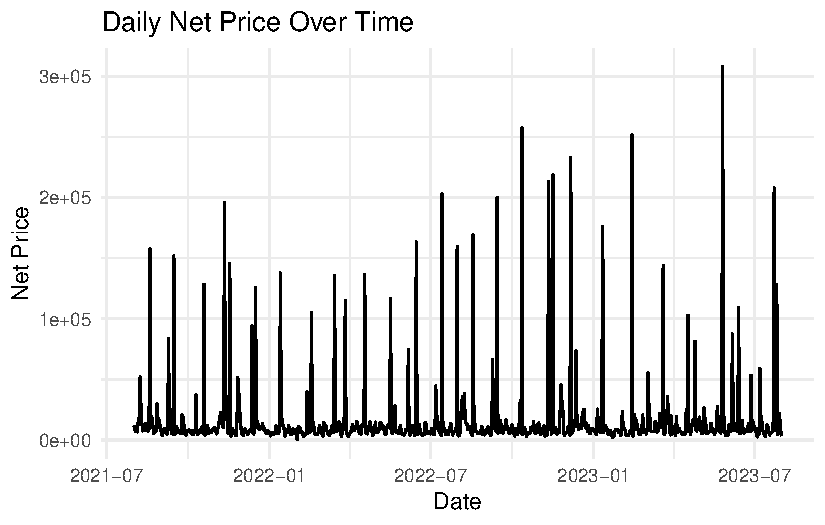
\includegraphics{Time-Serise-EDA_files/figure-pdf/unnamed-chunk-1-1.pdf}

}

\end{figure}

\begin{Shaded}
\begin{Highlighting}[]
\CommentTok{\# 计算Recency, Frequency, Monetary}
\NormalTok{df}\SpecialCharTok{$}\NormalTok{Recency }\OtherTok{\textless{}{-}} \FunctionTok{as.numeric}\NormalTok{(}\FunctionTok{difftime}\NormalTok{(}\FunctionTok{max}\NormalTok{(df}\SpecialCharTok{$}\StringTok{\textasciigrave{}}\AttributeTok{Document Date}\StringTok{\textasciigrave{}}\NormalTok{), df}\SpecialCharTok{$}\StringTok{\textasciigrave{}}\AttributeTok{Document Date}\StringTok{\textasciigrave{}}\NormalTok{, }\AttributeTok{units =} \StringTok{"days"}\NormalTok{))}

\NormalTok{df\_rfm }\OtherTok{\textless{}{-}}\NormalTok{ df }\SpecialCharTok{\%\textgreater{}\%}
  \FunctionTok{group\_by}\NormalTok{(Customer) }\SpecialCharTok{\%\textgreater{}\%}
  \FunctionTok{summarise}\NormalTok{(}
    \AttributeTok{Recency =} \FunctionTok{min}\NormalTok{(Recency, }\AttributeTok{na.rm =} \ConstantTok{TRUE}\NormalTok{),}
    \AttributeTok{Frequency =} \FunctionTok{n\_distinct}\NormalTok{(}\StringTok{\textasciigrave{}}\AttributeTok{Order No}\StringTok{\textasciigrave{}}\NormalTok{),}
    \AttributeTok{Monetary =} \FunctionTok{sum}\NormalTok{(}\StringTok{\textasciigrave{}}\AttributeTok{Net Price}\StringTok{\textasciigrave{}}\NormalTok{, }\AttributeTok{na.rm =} \ConstantTok{TRUE}\NormalTok{)}
\NormalTok{  )}

\FunctionTok{print}\NormalTok{(}\FunctionTok{head}\NormalTok{(df\_rfm))}
\end{Highlighting}
\end{Shaded}

\begin{verbatim}
# A tibble: 6 x 4
  Customer Recency Frequency Monetary
     <int>   <dbl>     <int>    <dbl>
1  1000003     693         1     46.7
2  1000147     678         1     23.4
3  1000298     587         1     34.6
4  1000343     725         1    105. 
5  1000467      57         1    219. 
6  1000468     231         1    433. 
\end{verbatim}

\begin{Shaded}
\begin{Highlighting}[]
\CommentTok{\# 示例产品代码}
\NormalTok{article\_code }\OtherTok{\textless{}{-}} \StringTok{"A14Y010000"}  \CommentTok{\# 替换为你的产品代码}

\CommentTok{\# 筛选指定产品的数据}
\NormalTok{df\_product }\OtherTok{\textless{}{-}}\NormalTok{ df }\SpecialCharTok{\%\textgreater{}\%}
  \FunctionTok{filter}\NormalTok{(}\StringTok{\textasciigrave{}}\AttributeTok{Article Code}\StringTok{\textasciigrave{}} \SpecialCharTok{==}\NormalTok{ article\_code) }\SpecialCharTok{\%\textgreater{}\%}
  \FunctionTok{group\_by}\NormalTok{(}\StringTok{\textasciigrave{}}\AttributeTok{Document Date}\StringTok{\textasciigrave{}}\NormalTok{, }\StringTok{\textasciigrave{}}\AttributeTok{Item Discount}\StringTok{\textasciigrave{}}\NormalTok{) }\SpecialCharTok{\%\textgreater{}\%}
  \FunctionTok{summarise}\NormalTok{(}\AttributeTok{Qty =} \FunctionTok{sum}\NormalTok{(Qty, }\AttributeTok{na.rm =} \ConstantTok{TRUE}\NormalTok{)) }\SpecialCharTok{\%\textgreater{}\%}
  \FunctionTok{ungroup}\NormalTok{()}
\end{Highlighting}
\end{Shaded}

\begin{verbatim}
`summarise()` has grouped output by 'Document Date'. You can override using the
`.groups` argument.
\end{verbatim}

\begin{Shaded}
\begin{Highlighting}[]
\CommentTok{\# 绘制产品销售情况}
\FunctionTok{ggplot}\NormalTok{(df\_product, }\FunctionTok{aes}\NormalTok{(}\AttributeTok{x =} \StringTok{\textasciigrave{}}\AttributeTok{Document Date}\StringTok{\textasciigrave{}}\NormalTok{, }\AttributeTok{y =}\NormalTok{ Qty)) }\SpecialCharTok{+}
  \FunctionTok{geom\_line}\NormalTok{() }\SpecialCharTok{+}
  \FunctionTok{geom\_point}\NormalTok{(}\AttributeTok{data =}\NormalTok{ df\_product }\SpecialCharTok{\%\textgreater{}\%} \FunctionTok{filter}\NormalTok{(}\StringTok{\textasciigrave{}}\AttributeTok{Item Discount}\StringTok{\textasciigrave{}} \SpecialCharTok{\textgreater{}} \DecValTok{0}\NormalTok{), }\FunctionTok{aes}\NormalTok{(}\AttributeTok{color =} \StringTok{"red"}\NormalTok{)) }\SpecialCharTok{+}
  \FunctionTok{scale\_color\_manual}\NormalTok{(}\AttributeTok{values =} \FunctionTok{c}\NormalTok{(}\StringTok{"red"} \OtherTok{=} \StringTok{"red"}\NormalTok{)) }\SpecialCharTok{+}
  \FunctionTok{labs}\NormalTok{(}\AttributeTok{title =} \FunctionTok{paste}\NormalTok{(}\StringTok{"Time Series Chart for Article Code:"}\NormalTok{, article\_code),}
       \AttributeTok{x =} \StringTok{"Document Date"}\NormalTok{, }\AttributeTok{y =} \StringTok{"Qty"}\NormalTok{,}
       \AttributeTok{color =} \StringTok{"Item on Discount"}\NormalTok{) }\SpecialCharTok{+}
  \FunctionTok{theme\_minimal}\NormalTok{()}
\end{Highlighting}
\end{Shaded}

\begin{verbatim}
Warning in grid.Call(C_textBounds, as.graphicsAnnot(x$label), x$x, x$y, :
conversion failure on '10月 2021' in 'mbcsToSbcs': dot substituted for <e6>
\end{verbatim}

\begin{verbatim}
Warning in grid.Call(C_textBounds, as.graphicsAnnot(x$label), x$x, x$y, :
conversion failure on '10月 2021' in 'mbcsToSbcs': dot substituted for <9c>
\end{verbatim}

\begin{verbatim}
Warning in grid.Call(C_textBounds, as.graphicsAnnot(x$label), x$x, x$y, :
conversion failure on '10月 2021' in 'mbcsToSbcs': dot substituted for <88>
\end{verbatim}

\begin{verbatim}
Warning in grid.Call(C_textBounds, as.graphicsAnnot(x$label), x$x, x$y, :
conversion failure on '1月 2022' in 'mbcsToSbcs': dot substituted for <e6>
\end{verbatim}

\begin{verbatim}
Warning in grid.Call(C_textBounds, as.graphicsAnnot(x$label), x$x, x$y, :
conversion failure on '1月 2022' in 'mbcsToSbcs': dot substituted for <9c>
\end{verbatim}

\begin{verbatim}
Warning in grid.Call(C_textBounds, as.graphicsAnnot(x$label), x$x, x$y, :
conversion failure on '1月 2022' in 'mbcsToSbcs': dot substituted for <88>
\end{verbatim}

\begin{verbatim}
Warning in grid.Call(C_textBounds, as.graphicsAnnot(x$label), x$x, x$y, :
conversion failure on '4月 2022' in 'mbcsToSbcs': dot substituted for <e6>
\end{verbatim}

\begin{verbatim}
Warning in grid.Call(C_textBounds, as.graphicsAnnot(x$label), x$x, x$y, :
conversion failure on '4月 2022' in 'mbcsToSbcs': dot substituted for <9c>
\end{verbatim}

\begin{verbatim}
Warning in grid.Call(C_textBounds, as.graphicsAnnot(x$label), x$x, x$y, :
conversion failure on '4月 2022' in 'mbcsToSbcs': dot substituted for <88>
\end{verbatim}

\begin{verbatim}
Warning in grid.Call(C_textBounds, as.graphicsAnnot(x$label), x$x, x$y, :
conversion failure on '7月 2022' in 'mbcsToSbcs': dot substituted for <e6>
\end{verbatim}

\begin{verbatim}
Warning in grid.Call(C_textBounds, as.graphicsAnnot(x$label), x$x, x$y, :
conversion failure on '7月 2022' in 'mbcsToSbcs': dot substituted for <9c>
\end{verbatim}

\begin{verbatim}
Warning in grid.Call(C_textBounds, as.graphicsAnnot(x$label), x$x, x$y, :
conversion failure on '7月 2022' in 'mbcsToSbcs': dot substituted for <88>
\end{verbatim}

\begin{verbatim}
Warning in grid.Call(C_textBounds, as.graphicsAnnot(x$label), x$x, x$y, :
conversion failure on '10月 2022' in 'mbcsToSbcs': dot substituted for <e6>
\end{verbatim}

\begin{verbatim}
Warning in grid.Call(C_textBounds, as.graphicsAnnot(x$label), x$x, x$y, :
conversion failure on '10月 2022' in 'mbcsToSbcs': dot substituted for <9c>
\end{verbatim}

\begin{verbatim}
Warning in grid.Call(C_textBounds, as.graphicsAnnot(x$label), x$x, x$y, :
conversion failure on '10月 2022' in 'mbcsToSbcs': dot substituted for <88>
\end{verbatim}

\begin{verbatim}
Warning in grid.Call.graphics(C_text, as.graphicsAnnot(x$label), x$x, x$y, :
conversion failure on '10月 2021' in 'mbcsToSbcs': dot substituted for <e6>
\end{verbatim}

\begin{verbatim}
Warning in grid.Call.graphics(C_text, as.graphicsAnnot(x$label), x$x, x$y, :
conversion failure on '10月 2021' in 'mbcsToSbcs': dot substituted for <9c>
\end{verbatim}

\begin{verbatim}
Warning in grid.Call.graphics(C_text, as.graphicsAnnot(x$label), x$x, x$y, :
conversion failure on '10月 2021' in 'mbcsToSbcs': dot substituted for <88>
\end{verbatim}

\begin{verbatim}
Warning in grid.Call.graphics(C_text, as.graphicsAnnot(x$label), x$x, x$y, :
conversion failure on '1月 2022' in 'mbcsToSbcs': dot substituted for <e6>
\end{verbatim}

\begin{verbatim}
Warning in grid.Call.graphics(C_text, as.graphicsAnnot(x$label), x$x, x$y, :
conversion failure on '1月 2022' in 'mbcsToSbcs': dot substituted for <9c>
\end{verbatim}

\begin{verbatim}
Warning in grid.Call.graphics(C_text, as.graphicsAnnot(x$label), x$x, x$y, :
conversion failure on '1月 2022' in 'mbcsToSbcs': dot substituted for <88>
\end{verbatim}

\begin{verbatim}
Warning in grid.Call.graphics(C_text, as.graphicsAnnot(x$label), x$x, x$y, :
conversion failure on '4月 2022' in 'mbcsToSbcs': dot substituted for <e6>
\end{verbatim}

\begin{verbatim}
Warning in grid.Call.graphics(C_text, as.graphicsAnnot(x$label), x$x, x$y, :
conversion failure on '4月 2022' in 'mbcsToSbcs': dot substituted for <9c>
\end{verbatim}

\begin{verbatim}
Warning in grid.Call.graphics(C_text, as.graphicsAnnot(x$label), x$x, x$y, :
conversion failure on '4月 2022' in 'mbcsToSbcs': dot substituted for <88>
\end{verbatim}

\begin{verbatim}
Warning in grid.Call.graphics(C_text, as.graphicsAnnot(x$label), x$x, x$y, :
conversion failure on '7月 2022' in 'mbcsToSbcs': dot substituted for <e6>
\end{verbatim}

\begin{verbatim}
Warning in grid.Call.graphics(C_text, as.graphicsAnnot(x$label), x$x, x$y, :
conversion failure on '7月 2022' in 'mbcsToSbcs': dot substituted for <9c>
\end{verbatim}

\begin{verbatim}
Warning in grid.Call.graphics(C_text, as.graphicsAnnot(x$label), x$x, x$y, :
conversion failure on '7月 2022' in 'mbcsToSbcs': dot substituted for <88>
\end{verbatim}

\begin{verbatim}
Warning in grid.Call.graphics(C_text, as.graphicsAnnot(x$label), x$x, x$y, :
conversion failure on '10月 2022' in 'mbcsToSbcs': dot substituted for <e6>
\end{verbatim}

\begin{verbatim}
Warning in grid.Call.graphics(C_text, as.graphicsAnnot(x$label), x$x, x$y, :
conversion failure on '10月 2022' in 'mbcsToSbcs': dot substituted for <9c>
\end{verbatim}

\begin{verbatim}
Warning in grid.Call.graphics(C_text, as.graphicsAnnot(x$label), x$x, x$y, :
conversion failure on '10月 2022' in 'mbcsToSbcs': dot substituted for <88>
\end{verbatim}

\begin{figure}[H]

{\centering 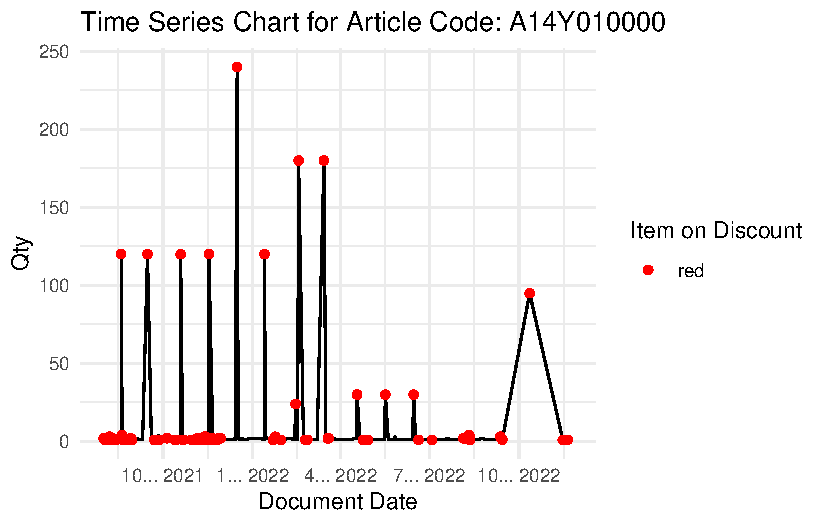
\includegraphics{Time-Serise-EDA_files/figure-pdf/unnamed-chunk-1-2.pdf}

}

\end{figure}

\begin{Shaded}
\begin{Highlighting}[]
\CommentTok{\# 计算每个产品是否增加销量}
\NormalTok{results\_df }\OtherTok{\textless{}{-}}\NormalTok{ df }\SpecialCharTok{\%\textgreater{}\%}
  \FunctionTok{group\_by}\NormalTok{(}\StringTok{\textasciigrave{}}\AttributeTok{Article Code}\StringTok{\textasciigrave{}}\NormalTok{, }\StringTok{\textasciigrave{}}\AttributeTok{Item Discount}\StringTok{\textasciigrave{}}\NormalTok{) }\SpecialCharTok{\%\textgreater{}\%}
  \FunctionTok{summarise}\NormalTok{(}\AttributeTok{Total\_Sales =} \FunctionTok{sum}\NormalTok{(Qty, }\AttributeTok{na.rm =} \ConstantTok{TRUE}\NormalTok{)) }\SpecialCharTok{\%\textgreater{}\%}
  \FunctionTok{pivot\_wider}\NormalTok{(}\AttributeTok{names\_from =} \StringTok{\textasciigrave{}}\AttributeTok{Item Discount}\StringTok{\textasciigrave{}}\NormalTok{, }\AttributeTok{values\_from =}\NormalTok{ Total\_Sales, }\AttributeTok{values\_fill =} \DecValTok{0}\NormalTok{) }\SpecialCharTok{\%\textgreater{}\%}
  \FunctionTok{mutate}\NormalTok{(}\AttributeTok{Increase\_in\_Sales =} \StringTok{\textasciigrave{}}\AttributeTok{1}\StringTok{\textasciigrave{}} \SpecialCharTok{\textgreater{}} \StringTok{\textasciigrave{}}\AttributeTok{0}\StringTok{\textasciigrave{}}\NormalTok{) }\SpecialCharTok{\%\textgreater{}\%}
  \FunctionTok{ungroup}\NormalTok{() }\SpecialCharTok{\%\textgreater{}\%}
  \FunctionTok{group\_by}\NormalTok{(Increase\_in\_Sales) }\SpecialCharTok{\%\textgreater{}\%}
  \FunctionTok{summarise}\NormalTok{(}\AttributeTok{Count =} \FunctionTok{n}\NormalTok{())}
\end{Highlighting}
\end{Shaded}

\begin{verbatim}
`summarise()` has grouped output by 'Article Code'. You can override using the
`.groups` argument.
\end{verbatim}

\begin{Shaded}
\begin{Highlighting}[]
\FunctionTok{print}\NormalTok{(}\FunctionTok{head}\NormalTok{(results\_df))}
\end{Highlighting}
\end{Shaded}

\begin{verbatim}
# A tibble: 1 x 2
  Increase_in_Sales Count
  <lgl>             <int>
1 FALSE               503
\end{verbatim}

\begin{Shaded}
\begin{Highlighting}[]
\CommentTok{\# 绘制分析结果}
\FunctionTok{ggplot}\NormalTok{(results\_df, }\FunctionTok{aes}\NormalTok{(}\AttributeTok{x =}\NormalTok{ Increase\_in\_Sales, }\AttributeTok{y =}\NormalTok{ Count, }\AttributeTok{fill =}\NormalTok{ Increase\_in\_Sales)) }\SpecialCharTok{+}
  \FunctionTok{geom\_bar}\NormalTok{(}\AttributeTok{stat =} \StringTok{"identity"}\NormalTok{) }\SpecialCharTok{+}
  \FunctionTok{labs}\NormalTok{(}\AttributeTok{title =} \StringTok{"Sales Increase Analysis"}\NormalTok{, }\AttributeTok{x =} \StringTok{"Increase in Sales"}\NormalTok{, }\AttributeTok{y =} \StringTok{"Count"}\NormalTok{) }\SpecialCharTok{+}
  \FunctionTok{theme\_minimal}\NormalTok{()}
\end{Highlighting}
\end{Shaded}

\begin{figure}[H]

{\centering 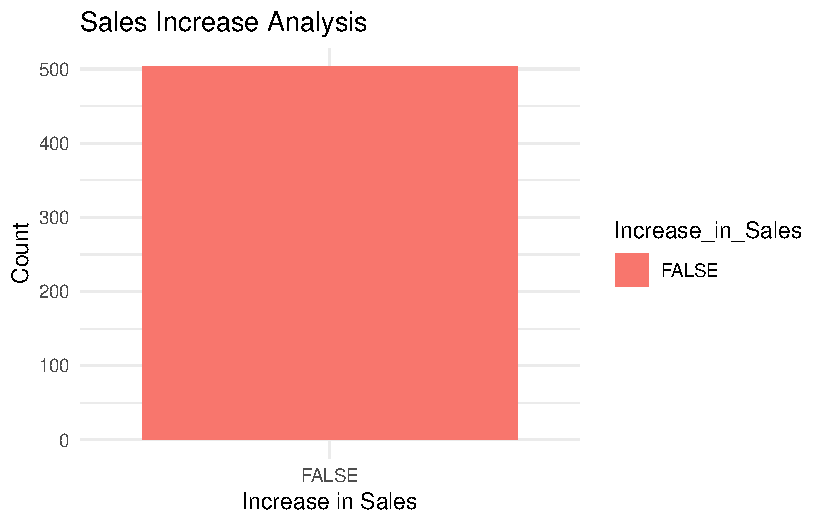
\includegraphics{Time-Serise-EDA_files/figure-pdf/unnamed-chunk-1-3.pdf}

}

\end{figure}

\begin{Shaded}
\begin{Highlighting}[]
\FunctionTok{library}\NormalTok{(tidyverse)}
\FunctionTok{library}\NormalTok{(lubridate)}
\FunctionTok{library}\NormalTok{(data.table)}
\FunctionTok{library}\NormalTok{(ggplot2)}
\FunctionTok{library}\NormalTok{(forecast)}
\end{Highlighting}
\end{Shaded}

\begin{verbatim}
Warning: package 'forecast' was built under R version 4.3.3
\end{verbatim}

\begin{verbatim}
Registered S3 method overwritten by 'quantmod':
  method            from
  as.zoo.data.frame zoo 
\end{verbatim}

\begin{Shaded}
\begin{Highlighting}[]
\CommentTok{\# 读取清洗后的数据}
\NormalTok{file\_path }\OtherTok{\textless{}{-}} \StringTok{"D:/cleaned\_transactions.csv"}  \CommentTok{\# 替换为清洗后数据的文件路径}
\NormalTok{df }\OtherTok{\textless{}{-}} \FunctionTok{fread}\NormalTok{(file\_path)}

\CommentTok{\# 解析日期}
\NormalTok{df}\SpecialCharTok{$}\StringTok{\textasciigrave{}}\AttributeTok{Document Date}\StringTok{\textasciigrave{}} \OtherTok{\textless{}{-}} \FunctionTok{as.Date}\NormalTok{(df}\SpecialCharTok{$}\StringTok{\textasciigrave{}}\AttributeTok{Document Date}\StringTok{\textasciigrave{}}\NormalTok{, }\AttributeTok{format =} \StringTok{"\%Y{-}\%m{-}\%d"}\NormalTok{)}

\CommentTok{\# 检查并移除无效日期}
\NormalTok{df }\OtherTok{\textless{}{-}}\NormalTok{ df }\SpecialCharTok{\%\textgreater{}\%}
  \FunctionTok{filter}\NormalTok{(}\SpecialCharTok{!}\FunctionTok{is.na}\NormalTok{(}\StringTok{\textasciigrave{}}\AttributeTok{Document Date}\StringTok{\textasciigrave{}}\NormalTok{))}

\CommentTok{\# 按日期聚合净价}
\NormalTok{df\_daily }\OtherTok{\textless{}{-}}\NormalTok{ df }\SpecialCharTok{\%\textgreater{}\%}
  \FunctionTok{group\_by}\NormalTok{(}\StringTok{\textasciigrave{}}\AttributeTok{Document Date}\StringTok{\textasciigrave{}}\NormalTok{) }\SpecialCharTok{\%\textgreater{}\%}
  \FunctionTok{summarise}\NormalTok{(}\AttributeTok{Net\_Price =} \FunctionTok{sum}\NormalTok{(}\StringTok{\textasciigrave{}}\AttributeTok{Net Price}\StringTok{\textasciigrave{}}\NormalTok{, }\AttributeTok{na.rm =} \ConstantTok{TRUE}\NormalTok{))}

\CommentTok{\# 按日期和分类聚合净价}
\NormalTok{df\_category\_daily }\OtherTok{\textless{}{-}}\NormalTok{ df }\SpecialCharTok{\%\textgreater{}\%}
  \FunctionTok{group\_by}\NormalTok{(}\StringTok{\textasciigrave{}}\AttributeTok{Document Date}\StringTok{\textasciigrave{}}\NormalTok{, }\StringTok{\textasciigrave{}}\AttributeTok{Category Description}\StringTok{\textasciigrave{}}\NormalTok{) }\SpecialCharTok{\%\textgreater{}\%}
  \FunctionTok{summarise}\NormalTok{(}\AttributeTok{Net\_Price =} \FunctionTok{sum}\NormalTok{(}\StringTok{\textasciigrave{}}\AttributeTok{Net Price}\StringTok{\textasciigrave{}}\NormalTok{, }\AttributeTok{na.rm =} \ConstantTok{TRUE}\NormalTok{)) }\SpecialCharTok{\%\textgreater{}\%}
  \FunctionTok{ungroup}\NormalTok{()}
\end{Highlighting}
\end{Shaded}

\begin{verbatim}
`summarise()` has grouped output by 'Document Date'. You can override using the
`.groups` argument.
\end{verbatim}

\begin{Shaded}
\begin{Highlighting}[]
\CommentTok{\# 按日期和销售渠道聚合净价}
\NormalTok{df\_channel\_daily }\OtherTok{\textless{}{-}}\NormalTok{ df }\SpecialCharTok{\%\textgreater{}\%}
  \FunctionTok{group\_by}\NormalTok{(}\StringTok{\textasciigrave{}}\AttributeTok{Document Date}\StringTok{\textasciigrave{}}\NormalTok{, }\StringTok{\textasciigrave{}}\AttributeTok{Sales Channel}\StringTok{\textasciigrave{}}\NormalTok{) }\SpecialCharTok{\%\textgreater{}\%}
  \FunctionTok{summarise}\NormalTok{(}\AttributeTok{Net\_Price =} \FunctionTok{sum}\NormalTok{(}\StringTok{\textasciigrave{}}\AttributeTok{Net Price}\StringTok{\textasciigrave{}}\NormalTok{, }\AttributeTok{na.rm =} \ConstantTok{TRUE}\NormalTok{)) }\SpecialCharTok{\%\textgreater{}\%}
  \FunctionTok{ungroup}\NormalTok{()}
\end{Highlighting}
\end{Shaded}

\begin{verbatim}
`summarise()` has grouped output by 'Document Date'. You can override using the
`.groups` argument.
\end{verbatim}

\begin{Shaded}
\begin{Highlighting}[]
\CommentTok{\# 绘制整体时间序列图}
\FunctionTok{ggplot}\NormalTok{(df\_daily, }\FunctionTok{aes}\NormalTok{(}\AttributeTok{x =} \StringTok{\textasciigrave{}}\AttributeTok{Document Date}\StringTok{\textasciigrave{}}\NormalTok{, }\AttributeTok{y =}\NormalTok{ Net\_Price)) }\SpecialCharTok{+}
  \FunctionTok{geom\_line}\NormalTok{() }\SpecialCharTok{+}
  \FunctionTok{labs}\NormalTok{(}\AttributeTok{title =} \StringTok{"Daily Net Price Over Time"}\NormalTok{,}
       \AttributeTok{x =} \StringTok{"Date"}\NormalTok{, }\AttributeTok{y =} \StringTok{"Net Price"}\NormalTok{) }\SpecialCharTok{+}
  \FunctionTok{theme\_minimal}\NormalTok{()}
\end{Highlighting}
\end{Shaded}

\begin{figure}[H]

{\centering 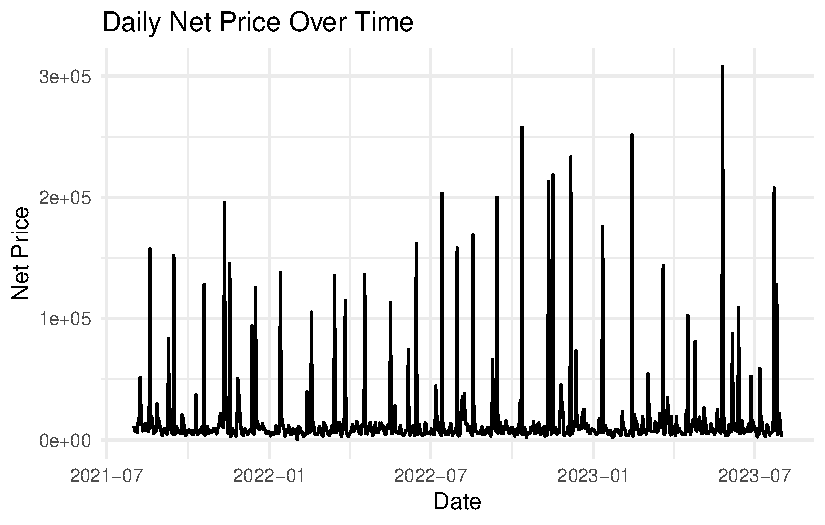
\includegraphics{Time-Serise-EDA_files/figure-pdf/unnamed-chunk-2-1.pdf}

}

\end{figure}

\begin{Shaded}
\begin{Highlighting}[]
\CommentTok{\# 绘制按分类的时间序列图}
\FunctionTok{ggplot}\NormalTok{(df\_category\_daily, }\FunctionTok{aes}\NormalTok{(}\AttributeTok{x =} \StringTok{\textasciigrave{}}\AttributeTok{Document Date}\StringTok{\textasciigrave{}}\NormalTok{, }\AttributeTok{y =}\NormalTok{ Net\_Price, }\AttributeTok{color =} \StringTok{\textasciigrave{}}\AttributeTok{Category Description}\StringTok{\textasciigrave{}}\NormalTok{)) }\SpecialCharTok{+}
  \FunctionTok{geom\_line}\NormalTok{() }\SpecialCharTok{+}
  \FunctionTok{labs}\NormalTok{(}\AttributeTok{title =} \StringTok{"Daily Net Price Over Time by Category"}\NormalTok{,}
       \AttributeTok{x =} \StringTok{"Date"}\NormalTok{, }\AttributeTok{y =} \StringTok{"Net Price"}\NormalTok{) }\SpecialCharTok{+}
  \FunctionTok{theme\_minimal}\NormalTok{() }\SpecialCharTok{+}
  \FunctionTok{theme}\NormalTok{(}\AttributeTok{legend.position =} \StringTok{"bottom"}\NormalTok{)}
\end{Highlighting}
\end{Shaded}

\begin{figure}[H]

{\centering 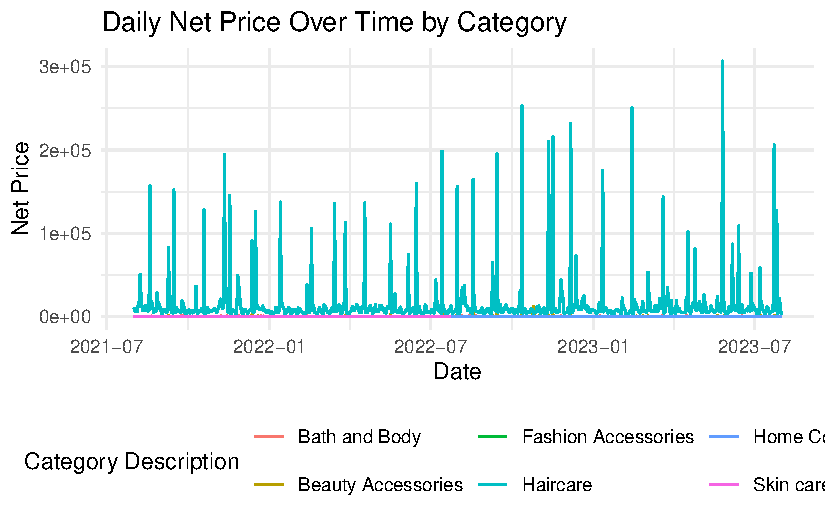
\includegraphics{Time-Serise-EDA_files/figure-pdf/unnamed-chunk-2-2.pdf}

}

\end{figure}

\begin{Shaded}
\begin{Highlighting}[]
\CommentTok{\# 绘制按销售渠道的时间序列图}
\FunctionTok{ggplot}\NormalTok{(df\_channel\_daily, }\FunctionTok{aes}\NormalTok{(}\AttributeTok{x =} \StringTok{\textasciigrave{}}\AttributeTok{Document Date}\StringTok{\textasciigrave{}}\NormalTok{, }\AttributeTok{y =}\NormalTok{ Net\_Price, }\AttributeTok{color =} \StringTok{\textasciigrave{}}\AttributeTok{Sales Channel}\StringTok{\textasciigrave{}}\NormalTok{)) }\SpecialCharTok{+}
  \FunctionTok{geom\_line}\NormalTok{() }\SpecialCharTok{+}
  \FunctionTok{labs}\NormalTok{(}\AttributeTok{title =} \StringTok{"Daily Net Price Over Time by Sales Channel"}\NormalTok{,}
       \AttributeTok{x =} \StringTok{"Date"}\NormalTok{, }\AttributeTok{y =} \StringTok{"Net Price"}\NormalTok{) }\SpecialCharTok{+}
  \FunctionTok{theme\_minimal}\NormalTok{() }\SpecialCharTok{+}
  \FunctionTok{theme}\NormalTok{(}\AttributeTok{legend.position =} \StringTok{"bottom"}\NormalTok{)}
\end{Highlighting}
\end{Shaded}

\begin{figure}[H]

{\centering 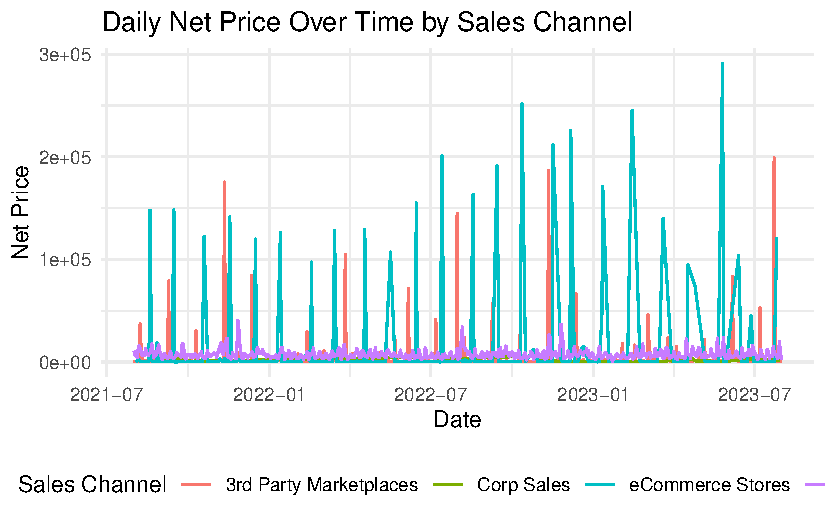
\includegraphics{Time-Serise-EDA_files/figure-pdf/unnamed-chunk-2-3.pdf}

}

\end{figure}

\begin{Shaded}
\begin{Highlighting}[]
\CommentTok{\# 按日期聚合销售数量}
\NormalTok{df\_qty\_daily }\OtherTok{\textless{}{-}}\NormalTok{ df }\SpecialCharTok{\%\textgreater{}\%}
  \FunctionTok{group\_by}\NormalTok{(}\StringTok{\textasciigrave{}}\AttributeTok{Document Date}\StringTok{\textasciigrave{}}\NormalTok{) }\SpecialCharTok{\%\textgreater{}\%}
  \FunctionTok{summarise}\NormalTok{(}\AttributeTok{Quantity =} \FunctionTok{sum}\NormalTok{(Qty, }\AttributeTok{na.rm =} \ConstantTok{TRUE}\NormalTok{))}

\CommentTok{\# 绘制销售数量时间序列图}
\FunctionTok{ggplot}\NormalTok{(df\_qty\_daily, }\FunctionTok{aes}\NormalTok{(}\AttributeTok{x =} \StringTok{\textasciigrave{}}\AttributeTok{Document Date}\StringTok{\textasciigrave{}}\NormalTok{, }\AttributeTok{y =}\NormalTok{ Quantity)) }\SpecialCharTok{+}
  \FunctionTok{geom\_line}\NormalTok{() }\SpecialCharTok{+}
  \FunctionTok{labs}\NormalTok{(}\AttributeTok{title =} \StringTok{"Daily Quantity Sold Over Time"}\NormalTok{,}
       \AttributeTok{x =} \StringTok{"Date"}\NormalTok{, }\AttributeTok{y =} \StringTok{"Quantity Sold"}\NormalTok{) }\SpecialCharTok{+}
  \FunctionTok{theme\_minimal}\NormalTok{()}
\end{Highlighting}
\end{Shaded}

\begin{figure}[H]

{\centering 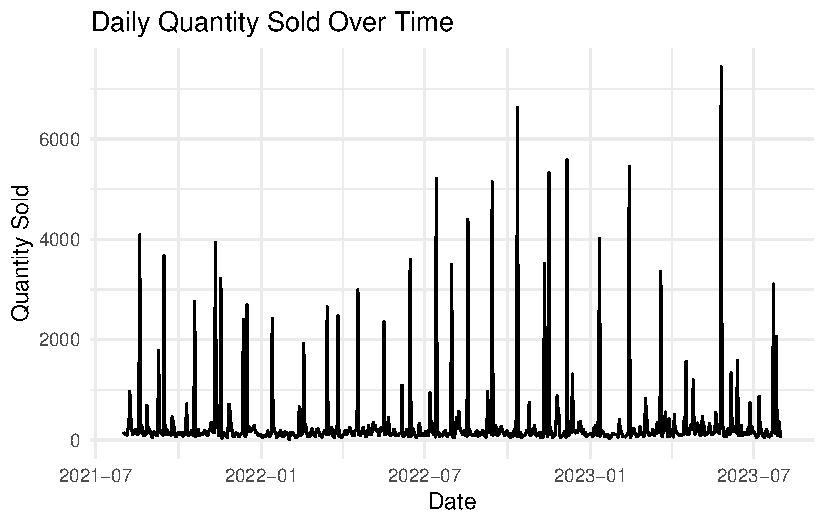
\includegraphics{Time-Serise-EDA_files/figure-pdf/unnamed-chunk-2-4.pdf}

}

\end{figure}

\begin{Shaded}
\begin{Highlighting}[]
\CommentTok{\# 按日期和折扣聚合净价}
\NormalTok{df\_discount\_daily }\OtherTok{\textless{}{-}}\NormalTok{ df }\SpecialCharTok{\%\textgreater{}\%}
  \FunctionTok{group\_by}\NormalTok{(}\StringTok{\textasciigrave{}}\AttributeTok{Document Date}\StringTok{\textasciigrave{}}\NormalTok{, Discount }\SpecialCharTok{\textgreater{}} \DecValTok{0}\NormalTok{) }\SpecialCharTok{\%\textgreater{}\%}
  \FunctionTok{summarise}\NormalTok{(}\AttributeTok{Net\_Price =} \FunctionTok{sum}\NormalTok{(}\StringTok{\textasciigrave{}}\AttributeTok{Net Price}\StringTok{\textasciigrave{}}\NormalTok{, }\AttributeTok{na.rm =} \ConstantTok{TRUE}\NormalTok{)) }\SpecialCharTok{\%\textgreater{}\%}
  \FunctionTok{ungroup}\NormalTok{() }\SpecialCharTok{\%\textgreater{}\%}
  \FunctionTok{mutate}\NormalTok{(}\AttributeTok{Discount\_Status =} \FunctionTok{ifelse}\NormalTok{(}\StringTok{\textasciigrave{}}\AttributeTok{Discount \textgreater{} 0}\StringTok{\textasciigrave{}}\NormalTok{, }\StringTok{"With Discount"}\NormalTok{, }\StringTok{"Without Discount"}\NormalTok{))}
\end{Highlighting}
\end{Shaded}

\begin{verbatim}
`summarise()` has grouped output by 'Document Date'. You can override using the
`.groups` argument.
\end{verbatim}

\begin{Shaded}
\begin{Highlighting}[]
\CommentTok{\# 绘制按折扣状态的时间序列图}
\FunctionTok{ggplot}\NormalTok{(df\_discount\_daily, }\FunctionTok{aes}\NormalTok{(}\AttributeTok{x =} \StringTok{\textasciigrave{}}\AttributeTok{Document Date}\StringTok{\textasciigrave{}}\NormalTok{, }\AttributeTok{y =}\NormalTok{ Net\_Price, }\AttributeTok{color =}\NormalTok{ Discount\_Status)) }\SpecialCharTok{+}
  \FunctionTok{geom\_line}\NormalTok{() }\SpecialCharTok{+}
  \FunctionTok{labs}\NormalTok{(}\AttributeTok{title =} \StringTok{"Daily Net Price Over Time by Discount Status"}\NormalTok{,}
       \AttributeTok{x =} \StringTok{"Date"}\NormalTok{, }\AttributeTok{y =} \StringTok{"Net Price"}\NormalTok{) }\SpecialCharTok{+}
  \FunctionTok{theme\_minimal}\NormalTok{() }\SpecialCharTok{+}
  \FunctionTok{theme}\NormalTok{(}\AttributeTok{legend.position =} \StringTok{"bottom"}\NormalTok{)}
\end{Highlighting}
\end{Shaded}

\begin{figure}[H]

{\centering 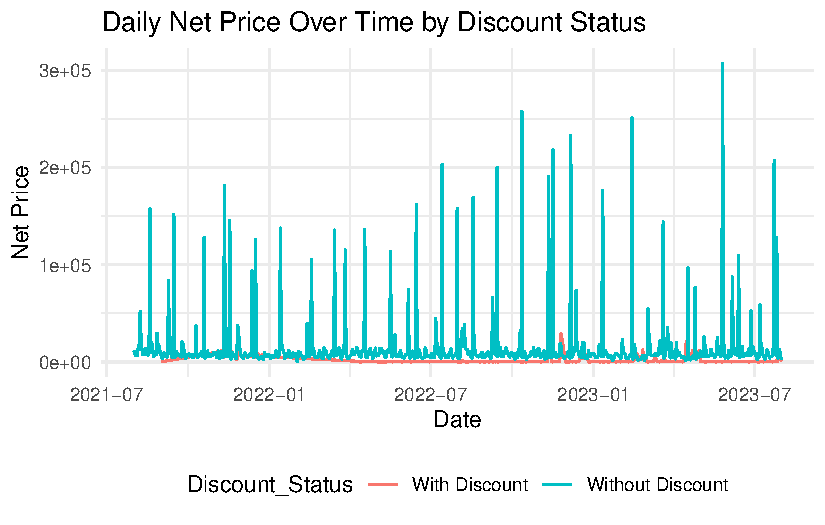
\includegraphics{Time-Serise-EDA_files/figure-pdf/unnamed-chunk-2-5.pdf}

}

\end{figure}

\begin{Shaded}
\begin{Highlighting}[]
\CommentTok{\# 季节性分解}
\NormalTok{ts\_net\_price }\OtherTok{\textless{}{-}} \FunctionTok{ts}\NormalTok{(df\_daily}\SpecialCharTok{$}\NormalTok{Net\_Price, }\AttributeTok{frequency =} \DecValTok{365}\NormalTok{)}
\NormalTok{decomp }\OtherTok{\textless{}{-}} \FunctionTok{decompose}\NormalTok{(ts\_net\_price)}
\FunctionTok{plot}\NormalTok{(decomp)}
\end{Highlighting}
\end{Shaded}

\begin{figure}[H]

{\centering 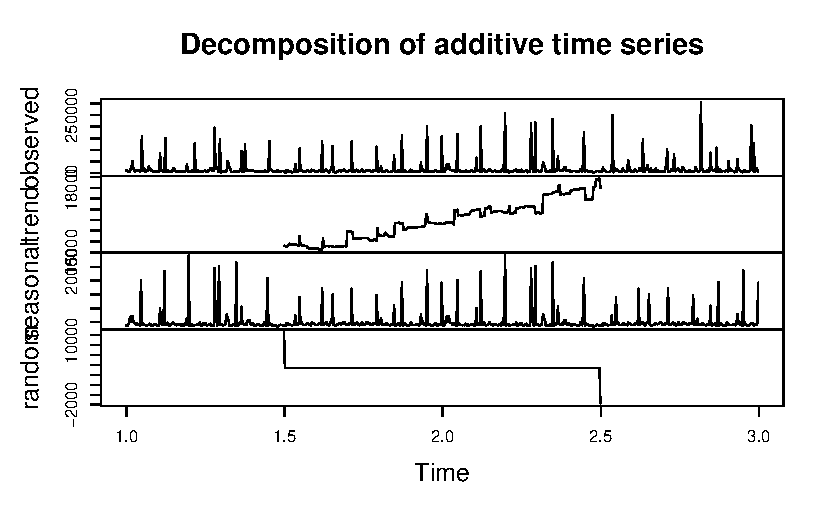
\includegraphics{Time-Serise-EDA_files/figure-pdf/unnamed-chunk-2-6.pdf}

}

\end{figure}

\begin{Shaded}
\begin{Highlighting}[]
\CommentTok{\# 按月聚合净价}
\NormalTok{df\_monthly }\OtherTok{\textless{}{-}}\NormalTok{ df\_daily }\SpecialCharTok{\%\textgreater{}\%}
  \FunctionTok{mutate}\NormalTok{(}\AttributeTok{Month =} \FunctionTok{floor\_date}\NormalTok{(}\StringTok{\textasciigrave{}}\AttributeTok{Document Date}\StringTok{\textasciigrave{}}\NormalTok{, }\StringTok{"month"}\NormalTok{)) }\SpecialCharTok{\%\textgreater{}\%}
  \FunctionTok{group\_by}\NormalTok{(Month) }\SpecialCharTok{\%\textgreater{}\%}
  \FunctionTok{summarise}\NormalTok{(}\AttributeTok{Net\_Price =} \FunctionTok{sum}\NormalTok{(Net\_Price, }\AttributeTok{na.rm =} \ConstantTok{TRUE}\NormalTok{))}

\CommentTok{\# 创建时间序列对象,频率设为12(表示每年12个时间点,即按月)}
\NormalTok{ts\_net\_price\_monthly }\OtherTok{\textless{}{-}} \FunctionTok{ts}\NormalTok{(df\_monthly}\SpecialCharTok{$}\NormalTok{Net\_Price, }\AttributeTok{start =} \FunctionTok{c}\NormalTok{(}\FunctionTok{year}\NormalTok{(}\FunctionTok{min}\NormalTok{(df\_monthly}\SpecialCharTok{$}\NormalTok{Month)), }\FunctionTok{month}\NormalTok{(}\FunctionTok{min}\NormalTok{(df\_monthly}\SpecialCharTok{$}\NormalTok{Month))), }\AttributeTok{frequency =} \DecValTok{12}\NormalTok{)}

\CommentTok{\# ACF图}
\FunctionTok{ggAcf}\NormalTok{(ts\_net\_price\_monthly) }\SpecialCharTok{+}
  \FunctionTok{labs}\NormalTok{(}\AttributeTok{title =} \StringTok{"ACF of Net Price (Monthly)"}\NormalTok{,}
       \AttributeTok{x =} \StringTok{"Month"}\NormalTok{, }\AttributeTok{y =} \StringTok{"ACF"}\NormalTok{) }\SpecialCharTok{+}
  \FunctionTok{scale\_x\_continuous}\NormalTok{(}\AttributeTok{breaks =} \FunctionTok{seq}\NormalTok{(}\DecValTok{0}\NormalTok{, }\DecValTok{24}\NormalTok{, }\DecValTok{3}\NormalTok{), }\AttributeTok{labels =} \ControlFlowTok{function}\NormalTok{(x) }\FunctionTok{format}\NormalTok{(}\FunctionTok{seq.Date}\NormalTok{(}\AttributeTok{from =} \FunctionTok{min}\NormalTok{(df\_monthly}\SpecialCharTok{$}\NormalTok{Month), }\AttributeTok{by =} \StringTok{"month"}\NormalTok{, }\AttributeTok{length.out =} \DecValTok{25}\NormalTok{)[x}\SpecialCharTok{+}\DecValTok{1}\NormalTok{], }\StringTok{"\%Y{-}\%m"}\NormalTok{))}
\end{Highlighting}
\end{Shaded}

\begin{verbatim}
Scale for x is already present.
Adding another scale for x, which will replace the existing scale.
\end{verbatim}

\begin{figure}[H]

{\centering 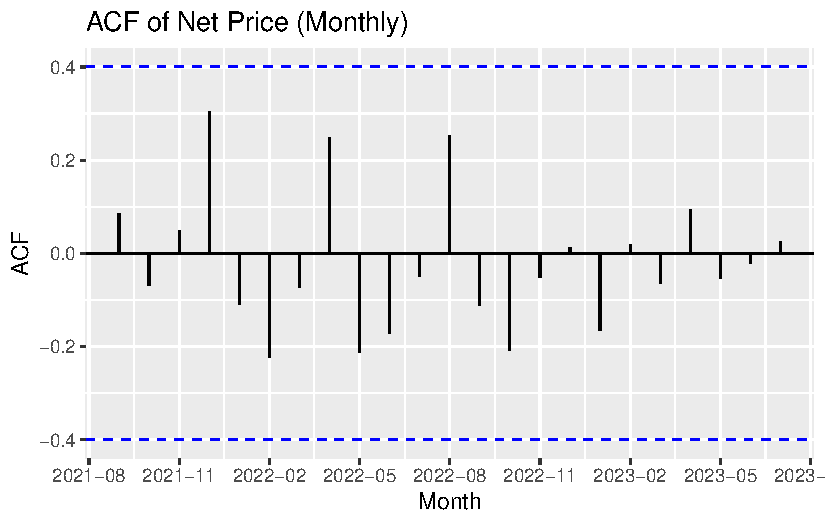
\includegraphics{Time-Serise-EDA_files/figure-pdf/unnamed-chunk-3-1.pdf}

}

\end{figure}

\begin{Shaded}
\begin{Highlighting}[]
\CommentTok{\# PACF图}
\FunctionTok{ggPacf}\NormalTok{(ts\_net\_price\_monthly) }\SpecialCharTok{+}
  \FunctionTok{labs}\NormalTok{(}\AttributeTok{title =} \StringTok{"PACF of Net Price (Monthly)"}\NormalTok{,}
       \AttributeTok{x =} \StringTok{"Month"}\NormalTok{, }\AttributeTok{y =} \StringTok{"PACF"}\NormalTok{) }\SpecialCharTok{+}
  \FunctionTok{scale\_x\_continuous}\NormalTok{(}\AttributeTok{breaks =} \FunctionTok{seq}\NormalTok{(}\DecValTok{0}\NormalTok{, }\DecValTok{24}\NormalTok{, }\DecValTok{3}\NormalTok{), }\AttributeTok{labels =} \ControlFlowTok{function}\NormalTok{(x) }\FunctionTok{format}\NormalTok{(}\FunctionTok{seq.Date}\NormalTok{(}\AttributeTok{from =} \FunctionTok{min}\NormalTok{(df\_monthly}\SpecialCharTok{$}\NormalTok{Month), }\AttributeTok{by =} \StringTok{"month"}\NormalTok{, }\AttributeTok{length.out =} \DecValTok{25}\NormalTok{)[x}\SpecialCharTok{+}\DecValTok{1}\NormalTok{], }\StringTok{"\%Y{-}\%m"}\NormalTok{))}
\end{Highlighting}
\end{Shaded}

\begin{verbatim}
Scale for x is already present.
Adding another scale for x, which will replace the existing scale.
\end{verbatim}

\begin{figure}[H]

{\centering 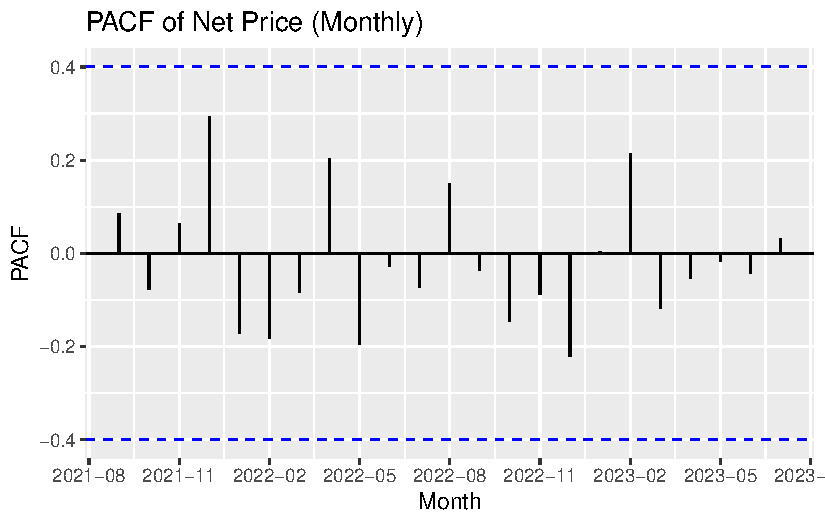
\includegraphics{Time-Serise-EDA_files/figure-pdf/unnamed-chunk-3-2.pdf}

}

\end{figure}

\begin{Shaded}
\begin{Highlighting}[]
\NormalTok{pacman}\SpecialCharTok{::}\FunctionTok{p\_load}\NormalTok{(prophet,seasonal,forecast,gridExtra)}
\end{Highlighting}
\end{Shaded}

\begin{Shaded}
\begin{Highlighting}[]
\FunctionTok{library}\NormalTok{(tidyverse)}
\FunctionTok{library}\NormalTok{(lubridate)}
\FunctionTok{library}\NormalTok{(data.table)}
\FunctionTok{library}\NormalTok{(ggplot2)}
\FunctionTok{library}\NormalTok{(forecast)}
\FunctionTok{library}\NormalTok{(gridExtra)}
\FunctionTok{library}\NormalTok{(scales)}
\end{Highlighting}
\end{Shaded}

\begin{verbatim}

Attaching package: 'scales'
\end{verbatim}

\begin{verbatim}
The following object is masked from 'package:purrr':

    discard
\end{verbatim}

\begin{verbatim}
The following object is masked from 'package:readr':

    col_factor
\end{verbatim}

\begin{Shaded}
\begin{Highlighting}[]
\CommentTok{\# 读取清洗后的数据}
\NormalTok{file\_path }\OtherTok{\textless{}{-}} \StringTok{"D:/cleaned\_transactions.csv"}  \CommentTok{\# 替换为清洗后数据的文件路径}
\NormalTok{df }\OtherTok{\textless{}{-}} \FunctionTok{fread}\NormalTok{(file\_path)}

\CommentTok{\# 解析日期}
\NormalTok{df}\SpecialCharTok{$}\StringTok{\textasciigrave{}}\AttributeTok{Document Date}\StringTok{\textasciigrave{}} \OtherTok{\textless{}{-}} \FunctionTok{as.Date}\NormalTok{(df}\SpecialCharTok{$}\StringTok{\textasciigrave{}}\AttributeTok{Document Date}\StringTok{\textasciigrave{}}\NormalTok{, }\AttributeTok{format =} \StringTok{"\%Y{-}\%m{-}\%d"}\NormalTok{)}

\CommentTok{\# 按日期聚合净价}
\NormalTok{df\_daily }\OtherTok{\textless{}{-}}\NormalTok{ df }\SpecialCharTok{\%\textgreater{}\%}
  \FunctionTok{group\_by}\NormalTok{(}\StringTok{\textasciigrave{}}\AttributeTok{Document Date}\StringTok{\textasciigrave{}}\NormalTok{) }\SpecialCharTok{\%\textgreater{}\%}
  \FunctionTok{summarise}\NormalTok{(}\AttributeTok{Net\_Price =} \FunctionTok{sum}\NormalTok{(}\StringTok{\textasciigrave{}}\AttributeTok{Net Price}\StringTok{\textasciigrave{}}\NormalTok{, }\AttributeTok{na.rm =} \ConstantTok{TRUE}\NormalTok{))}

\CommentTok{\# 确保日期序列连续}
\NormalTok{df\_daily }\OtherTok{\textless{}{-}}\NormalTok{ df\_daily }\SpecialCharTok{\%\textgreater{}\%}
  \FunctionTok{complete}\NormalTok{(}\StringTok{\textasciigrave{}}\AttributeTok{Document Date}\StringTok{\textasciigrave{}} \OtherTok{=} \FunctionTok{seq.Date}\NormalTok{(}\FunctionTok{min}\NormalTok{(}\StringTok{\textasciigrave{}}\AttributeTok{Document Date}\StringTok{\textasciigrave{}}\NormalTok{), }\FunctionTok{max}\NormalTok{(}\StringTok{\textasciigrave{}}\AttributeTok{Document Date}\StringTok{\textasciigrave{}}\NormalTok{), }\AttributeTok{by =} \StringTok{"day"}\NormalTok{)) }\SpecialCharTok{\%\textgreater{}\%}
  \FunctionTok{fill}\NormalTok{(Net\_Price, }\AttributeTok{.direction =} \StringTok{"downup"}\NormalTok{)}

\CommentTok{\# 创建时间序列对象,指定开始和结束日期}
\NormalTok{start\_date }\OtherTok{\textless{}{-}} \FunctionTok{as.numeric}\NormalTok{(}\FunctionTok{format}\NormalTok{(}\FunctionTok{min}\NormalTok{(df\_daily}\SpecialCharTok{$}\StringTok{\textasciigrave{}}\AttributeTok{Document Date}\StringTok{\textasciigrave{}}\NormalTok{), }\StringTok{"\%Y"}\NormalTok{))}
\NormalTok{start\_month }\OtherTok{\textless{}{-}} \FunctionTok{as.numeric}\NormalTok{(}\FunctionTok{format}\NormalTok{(}\FunctionTok{min}\NormalTok{(df\_daily}\SpecialCharTok{$}\StringTok{\textasciigrave{}}\AttributeTok{Document Date}\StringTok{\textasciigrave{}}\NormalTok{), }\StringTok{"\%m"}\NormalTok{))}
\NormalTok{ts\_net\_price }\OtherTok{\textless{}{-}} \FunctionTok{ts}\NormalTok{(df\_daily}\SpecialCharTok{$}\NormalTok{Net\_Price, }\AttributeTok{start =} \FunctionTok{c}\NormalTok{(start\_date, start\_month), }\AttributeTok{frequency =} \DecValTok{365}\NormalTok{)}

\CommentTok{\# 季节性分解}
\NormalTok{decomp }\OtherTok{\textless{}{-}} \FunctionTok{decompose}\NormalTok{(ts\_net\_price)}

\CommentTok{\# 使用 ggplot2 绘制分解结果}
\NormalTok{decomp\_df }\OtherTok{\textless{}{-}} \FunctionTok{data.frame}\NormalTok{(}
  \AttributeTok{date =} \FunctionTok{seq.Date}\NormalTok{(}\AttributeTok{from =} \FunctionTok{min}\NormalTok{(df\_daily}\SpecialCharTok{$}\StringTok{\textasciigrave{}}\AttributeTok{Document Date}\StringTok{\textasciigrave{}}\NormalTok{), }\AttributeTok{by =} \StringTok{"day"}\NormalTok{, }\AttributeTok{length.out =} \FunctionTok{length}\NormalTok{(decomp}\SpecialCharTok{$}\NormalTok{trend)),}
  \AttributeTok{observed =}\NormalTok{ decomp}\SpecialCharTok{$}\NormalTok{x,}
  \AttributeTok{trend =}\NormalTok{ decomp}\SpecialCharTok{$}\NormalTok{trend,}
  \AttributeTok{seasonal =}\NormalTok{ decomp}\SpecialCharTok{$}\NormalTok{seasonal,}
  \AttributeTok{random =}\NormalTok{ decomp}\SpecialCharTok{$}\NormalTok{random}
\NormalTok{)}

\NormalTok{p1 }\OtherTok{\textless{}{-}} \FunctionTok{ggplot}\NormalTok{(decomp\_df, }\FunctionTok{aes}\NormalTok{(}\AttributeTok{x =}\NormalTok{ date, }\AttributeTok{y =}\NormalTok{ observed)) }\SpecialCharTok{+}
  \FunctionTok{geom\_line}\NormalTok{(}\AttributeTok{color =} \StringTok{"blue"}\NormalTok{) }\SpecialCharTok{+}
  \FunctionTok{labs}\NormalTok{(}\AttributeTok{title =} \StringTok{"Observed"}\NormalTok{, }\AttributeTok{x =} \StringTok{"Date"}\NormalTok{, }\AttributeTok{y =} \StringTok{"Observed"}\NormalTok{) }\SpecialCharTok{+}
  \FunctionTok{scale\_y\_continuous}\NormalTok{(}\AttributeTok{labels =}\NormalTok{ scales}\SpecialCharTok{::}\NormalTok{comma) }\SpecialCharTok{+}
  \FunctionTok{theme\_minimal}\NormalTok{()}

\NormalTok{p2 }\OtherTok{\textless{}{-}} \FunctionTok{ggplot}\NormalTok{(decomp\_df, }\FunctionTok{aes}\NormalTok{(}\AttributeTok{x =}\NormalTok{ date, }\AttributeTok{y =}\NormalTok{ trend)) }\SpecialCharTok{+}
  \FunctionTok{geom\_line}\NormalTok{(}\AttributeTok{color =} \StringTok{"blue"}\NormalTok{) }\SpecialCharTok{+}
  \FunctionTok{labs}\NormalTok{(}\AttributeTok{title =} \StringTok{"Trend"}\NormalTok{, }\AttributeTok{x =} \StringTok{"Date"}\NormalTok{, }\AttributeTok{y =} \StringTok{"Trend"}\NormalTok{) }\SpecialCharTok{+}
  \FunctionTok{scale\_y\_continuous}\NormalTok{(}\AttributeTok{labels =}\NormalTok{ scales}\SpecialCharTok{::}\NormalTok{comma) }\SpecialCharTok{+}
  \FunctionTok{theme\_minimal}\NormalTok{()}

\NormalTok{p3 }\OtherTok{\textless{}{-}} \FunctionTok{ggplot}\NormalTok{(decomp\_df, }\FunctionTok{aes}\NormalTok{(}\AttributeTok{x =}\NormalTok{ date, }\AttributeTok{y =}\NormalTok{ seasonal)) }\SpecialCharTok{+}
  \FunctionTok{geom\_line}\NormalTok{(}\AttributeTok{color =} \StringTok{"blue"}\NormalTok{) }\SpecialCharTok{+}
  \FunctionTok{labs}\NormalTok{(}\AttributeTok{title =} \StringTok{"Seasonal"}\NormalTok{, }\AttributeTok{x =} \StringTok{"Date"}\NormalTok{, }\AttributeTok{y =} \StringTok{"Seasonal"}\NormalTok{) }\SpecialCharTok{+}
  \FunctionTok{scale\_y\_continuous}\NormalTok{(}\AttributeTok{labels =}\NormalTok{ scales}\SpecialCharTok{::}\NormalTok{comma) }\SpecialCharTok{+}
  \FunctionTok{theme\_minimal}\NormalTok{()}

\NormalTok{p4 }\OtherTok{\textless{}{-}} \FunctionTok{ggplot}\NormalTok{(decomp\_df, }\FunctionTok{aes}\NormalTok{(}\AttributeTok{x =}\NormalTok{ date, }\AttributeTok{y =}\NormalTok{ random)) }\SpecialCharTok{+}
  \FunctionTok{geom\_line}\NormalTok{(}\AttributeTok{color =} \StringTok{"blue"}\NormalTok{) }\SpecialCharTok{+}
  \FunctionTok{labs}\NormalTok{(}\AttributeTok{title =} \StringTok{"Random"}\NormalTok{, }\AttributeTok{x =} \StringTok{"Date"}\NormalTok{, }\AttributeTok{y =} \StringTok{"Random"}\NormalTok{) }\SpecialCharTok{+}
  \FunctionTok{scale\_y\_continuous}\NormalTok{(}\AttributeTok{labels =}\NormalTok{ scales}\SpecialCharTok{::}\NormalTok{comma) }\SpecialCharTok{+}
  \FunctionTok{theme\_minimal}\NormalTok{()}

\CommentTok{\# 使用 gridExtra 包将四个图放在一起}
\FunctionTok{grid.arrange}\NormalTok{(p1, p2, p3, p4, }\AttributeTok{ncol =} \DecValTok{1}\NormalTok{)}
\end{Highlighting}
\end{Shaded}

\begin{verbatim}
Warning: Removed 364 rows containing missing values or values outside the scale range
(`geom_line()`).
Removed 364 rows containing missing values or values outside the scale range
(`geom_line()`).
\end{verbatim}

\begin{figure}[H]

{\centering 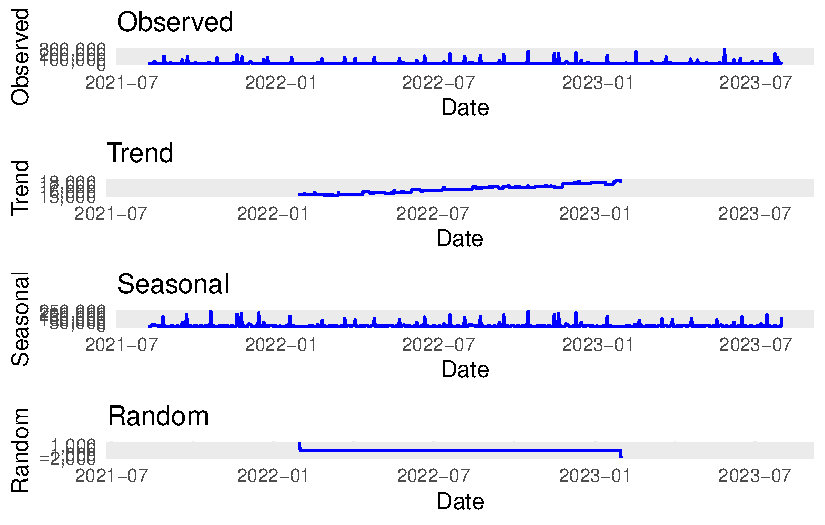
\includegraphics{Time-Serise-EDA_files/figure-pdf/unnamed-chunk-5-1.pdf}

}

\end{figure}

\begin{Shaded}
\begin{Highlighting}[]
\FunctionTok{library}\NormalTok{(tidyverse)}
\FunctionTok{library}\NormalTok{(data.table)}

\CommentTok{\# 读取数据}
\NormalTok{file\_path }\OtherTok{\textless{}{-}} \StringTok{"D:/transactions.csv"}  \CommentTok{\# 替换为你的文件路径}
\NormalTok{df }\OtherTok{\textless{}{-}} \FunctionTok{fread}\NormalTok{(file\_path)}

\CommentTok{\# 解析日期}
\NormalTok{df}\SpecialCharTok{$}\StringTok{\textasciigrave{}}\AttributeTok{Document Date}\StringTok{\textasciigrave{}} \OtherTok{\textless{}{-}} \FunctionTok{as.Date}\NormalTok{(df}\SpecialCharTok{$}\StringTok{\textasciigrave{}}\AttributeTok{Document Date}\StringTok{\textasciigrave{}}\NormalTok{, }\AttributeTok{format =} \StringTok{"\%m/\%d/\%Y"}\NormalTok{)}

\CommentTok{\# 新列:Item\_Type}
\NormalTok{df }\OtherTok{\textless{}{-}}\NormalTok{ df }\SpecialCharTok{\%\textgreater{}\%}
  \FunctionTok{mutate}\NormalTok{(}\AttributeTok{Item\_Type =} \FunctionTok{case\_when}\NormalTok{(}
    \StringTok{\textasciigrave{}}\AttributeTok{Net Price}\StringTok{\textasciigrave{}} \SpecialCharTok{==} \DecValTok{0} \SpecialCharTok{\&} \FunctionTok{str\_detect}\NormalTok{(Description, }\StringTok{"Sample|SP|SAMP|SMP"}\NormalTok{) }\SpecialCharTok{\textasciitilde{}} \StringTok{"Sample"}\NormalTok{,}
    \StringTok{\textasciigrave{}}\AttributeTok{Net Price}\StringTok{\textasciigrave{}} \SpecialCharTok{==} \DecValTok{0} \SpecialCharTok{\&} \FunctionTok{str\_detect}\NormalTok{(Description, }\StringTok{"GWP"}\NormalTok{) }\SpecialCharTok{\textasciitilde{}} \StringTok{"GWP"}\NormalTok{,}
    \ConstantTok{TRUE} \SpecialCharTok{\textasciitilde{}} \StringTok{"Paid"}
\NormalTok{  ))}

\CommentTok{\# 新列:Series}
\NormalTok{df }\OtherTok{\textless{}{-}}\NormalTok{ df }\SpecialCharTok{\%\textgreater{}\%}
  \FunctionTok{mutate}\NormalTok{(}\AttributeTok{Series =} \FunctionTok{case\_when}\NormalTok{(}
    \FunctionTok{str\_detect}\NormalTok{(Description, }\StringTok{"Invati"}\NormalTok{) }\SpecialCharTok{\textasciitilde{}} \StringTok{"Invati"}\NormalTok{,}
    \FunctionTok{str\_detect}\NormalTok{(Description, }\StringTok{"Botanical Repair"}\NormalTok{) }\SpecialCharTok{\textasciitilde{}} \StringTok{"Botanical Repair"}\NormalTok{,}
    \FunctionTok{str\_detect}\NormalTok{(Description, }\StringTok{"Colour Control"}\NormalTok{) }\SpecialCharTok{\textasciitilde{}} \StringTok{"Colour Control"}\NormalTok{,}
    \FunctionTok{str\_detect}\NormalTok{(Description, }\StringTok{"Rosemary Mint"}\NormalTok{) }\SpecialCharTok{\textasciitilde{}} \StringTok{"Rosemary Mint"}\NormalTok{,}
    \ConstantTok{TRUE} \SpecialCharTok{\textasciitilde{}} \StringTok{"Other"}
\NormalTok{  ))}

\CommentTok{\# 筛选 Sales\_Transaction = \textquotesingle{}S\textquotesingle{} 和 Item\_Type = \textquotesingle{}Paid\textquotesingle{} 的记录}
\NormalTok{df\_filtered }\OtherTok{\textless{}{-}}\NormalTok{ df }\SpecialCharTok{\%\textgreater{}\%}
  \FunctionTok{filter}\NormalTok{(}\StringTok{\textasciigrave{}}\AttributeTok{Sales Transaction Type}\StringTok{\textasciigrave{}} \SpecialCharTok{==} \StringTok{\textquotesingle{}S\textquotesingle{}} \SpecialCharTok{\&}\NormalTok{ Item\_Type }\SpecialCharTok{==} \StringTok{\textquotesingle{}Paid\textquotesingle{}}\NormalTok{)}

\CommentTok{\# 查看数据清洗后的结果}
\FunctionTok{head}\NormalTok{(df\_filtered)}
\end{Highlighting}
\end{Shaded}

\begin{verbatim}
     Order No Customer Sales Transaction Type Document Date Store Id
1: 3006716497  3616853                      S    2021-08-01     6022
2: 3006716497  3616853                      S    2021-08-01     6022
3: 3006716497  3616853                      S    2021-08-01     6022
4: 3006716498  2707866                      S    2021-08-01     5009
5: 3006716498  2707866                      S    2021-08-01     5009
6: 3006716498  2707866                      S    2021-08-01     5009
   Sales Employee Id Article Code                           Description
1:          20011149   AMFR010000       AVH INVATI ADV THICK COND 200ML
2:          20011149   AMFW010000    AVH INVATI ADV SCALP REVITAL 150ML
3:          20011149   AWLC010000   AVH INVATI ADV EXF SHAMP RICH 200ML
4:          20011525   A46M010000          AVH MENS FIRM HOLD GEL 150ML
5:          20011525   AKCH010000    AVH INVATI MEN SCALP REVITAL 125ML
6:          20011525   AWK8010000 AVH INVATI ADV EXF SHAMP LIGHT 1000ML
   Category Description Sales Channel Discount  Gst Item Discount Net Price Qty
1:             Haircare        Retail        0 3.66           0.0     52.34   1
2:             Haircare        Retail        0 7.99           0.0    114.01   1
3:             Haircare        Retail        0 3.53           0.0     50.47   1
4:             Haircare        Retail        0 3.27           0.0     46.73   1
5:             Haircare        Retail        0 7.33           0.0    104.67   1
6:             Haircare        Retail        0 9.73          37.2    139.07   1
   Retail Price Item_Type Series
1:           56      Paid  Other
2:          122      Paid  Other
3:           54      Paid  Other
4:           50      Paid  Other
5:          112      Paid  Other
6:          186      Paid  Other
\end{verbatim}

\begin{Shaded}
\begin{Highlighting}[]
\CommentTok{\# 按日期聚合净价}
\NormalTok{df\_daily }\OtherTok{\textless{}{-}}\NormalTok{ df\_filtered }\SpecialCharTok{\%\textgreater{}\%}
  \FunctionTok{group\_by}\NormalTok{(}\StringTok{\textasciigrave{}}\AttributeTok{Document Date}\StringTok{\textasciigrave{}}\NormalTok{) }\SpecialCharTok{\%\textgreater{}\%}
  \FunctionTok{summarise}\NormalTok{(}\AttributeTok{Net\_Price =} \FunctionTok{sum}\NormalTok{(}\StringTok{\textasciigrave{}}\AttributeTok{Net Price}\StringTok{\textasciigrave{}}\NormalTok{, }\AttributeTok{na.rm =} \ConstantTok{TRUE}\NormalTok{))}

\CommentTok{\# 绘制净价格为零的记录分布情况}
\NormalTok{zero\_net\_price\_records }\OtherTok{\textless{}{-}}\NormalTok{ df\_filtered }\SpecialCharTok{\%\textgreater{}\%}
  \FunctionTok{filter}\NormalTok{(}\StringTok{\textasciigrave{}}\AttributeTok{Net Price}\StringTok{\textasciigrave{}} \SpecialCharTok{==} \DecValTok{0}\NormalTok{)}

\CommentTok{\# 按销售渠道分组并计算数量}
\NormalTok{channel\_summary }\OtherTok{\textless{}{-}}\NormalTok{ zero\_net\_price\_records }\SpecialCharTok{\%\textgreater{}\%}
  \FunctionTok{group\_by}\NormalTok{(}\StringTok{\textasciigrave{}}\AttributeTok{Sales Channel}\StringTok{\textasciigrave{}}\NormalTok{) }\SpecialCharTok{\%\textgreater{}\%}
  \FunctionTok{summarise}\NormalTok{(}\AttributeTok{Count =} \FunctionTok{n}\NormalTok{())}

\CommentTok{\# 绘制条形图}
\FunctionTok{ggplot}\NormalTok{(channel\_summary, }\FunctionTok{aes}\NormalTok{(}\AttributeTok{x =} \StringTok{\textasciigrave{}}\AttributeTok{Sales Channel}\StringTok{\textasciigrave{}}\NormalTok{, }\AttributeTok{y =}\NormalTok{ Count, }\AttributeTok{fill =} \StringTok{\textasciigrave{}}\AttributeTok{Sales Channel}\StringTok{\textasciigrave{}}\NormalTok{)) }\SpecialCharTok{+}
  \FunctionTok{geom\_bar}\NormalTok{(}\AttributeTok{stat =} \StringTok{"identity"}\NormalTok{) }\SpecialCharTok{+}
  \FunctionTok{labs}\NormalTok{(}\AttributeTok{title =} \StringTok{"Zero Net Price Records by Sales Channel"}\NormalTok{,}
       \AttributeTok{x =} \StringTok{"Sales Channel"}\NormalTok{, }\AttributeTok{y =} \StringTok{"Count"}\NormalTok{) }\SpecialCharTok{+}
  \FunctionTok{theme\_minimal}\NormalTok{()}
\end{Highlighting}
\end{Shaded}

\begin{figure}[H]

{\centering 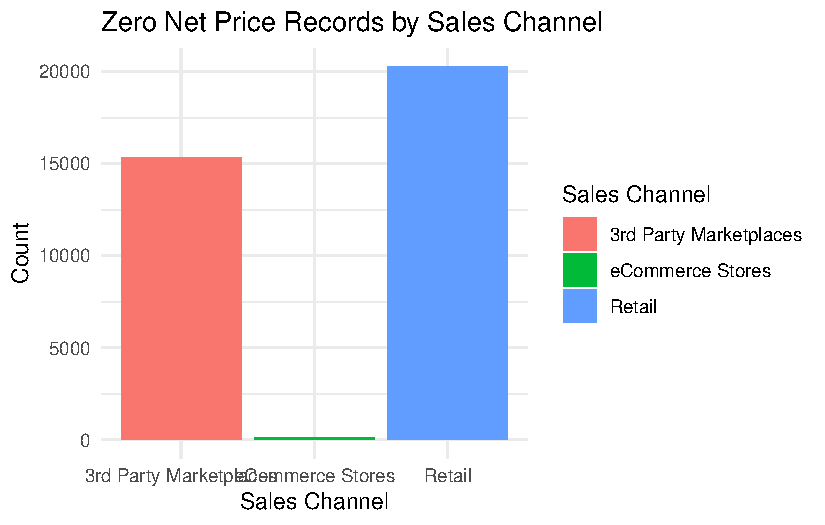
\includegraphics{Time-Serise-EDA_files/figure-pdf/unnamed-chunk-6-1.pdf}

}

\end{figure}

\begin{Shaded}
\begin{Highlighting}[]
\NormalTok{output\_file\_path }\OtherTok{\textless{}{-}} \StringTok{"D:/cleaned\_transactions.csv"}  \CommentTok{\# 替换为你希望保存文件的路径}
\FunctionTok{write.csv}\NormalTok{(df\_filtered, output\_file\_path, }\AttributeTok{row.names =} \ConstantTok{FALSE}\NormalTok{)}
\end{Highlighting}
\end{Shaded}

\begin{Shaded}
\begin{Highlighting}[]
\FunctionTok{library}\NormalTok{(tidyverse)}
\FunctionTok{library}\NormalTok{(lubridate)}
\FunctionTok{library}\NormalTok{(data.table)}
\FunctionTok{library}\NormalTok{(ggridges)}
\end{Highlighting}
\end{Shaded}

\begin{verbatim}
Warning: package 'ggridges' was built under R version 4.3.3
\end{verbatim}

\begin{Shaded}
\begin{Highlighting}[]
\FunctionTok{library}\NormalTok{(scales)}

\CommentTok{\# 解析日期}
\NormalTok{df}\SpecialCharTok{$}\StringTok{\textasciigrave{}}\AttributeTok{Document Date}\StringTok{\textasciigrave{}} \OtherTok{\textless{}{-}} \FunctionTok{as.Date}\NormalTok{(df}\SpecialCharTok{$}\StringTok{\textasciigrave{}}\AttributeTok{Document Date}\StringTok{\textasciigrave{}}\NormalTok{, }\AttributeTok{format =} \StringTok{"\%Y{-}\%m{-}\%d"}\NormalTok{)}

\CommentTok{\# 按日期和分类聚合净价}
\NormalTok{df\_category\_daily }\OtherTok{\textless{}{-}}\NormalTok{ df }\SpecialCharTok{\%\textgreater{}\%}
  \FunctionTok{filter}\NormalTok{(}\StringTok{\textasciigrave{}}\AttributeTok{Sales Transaction Type}\StringTok{\textasciigrave{}} \SpecialCharTok{==} \StringTok{"S"}\NormalTok{, }\StringTok{\textasciigrave{}}\AttributeTok{Item\_Type}\StringTok{\textasciigrave{}} \SpecialCharTok{==} \StringTok{"Paid"}\NormalTok{) }\SpecialCharTok{\%\textgreater{}\%}
  \FunctionTok{group\_by}\NormalTok{(}\StringTok{\textasciigrave{}}\AttributeTok{Document Date}\StringTok{\textasciigrave{}}\NormalTok{, }\StringTok{\textasciigrave{}}\AttributeTok{Category Description}\StringTok{\textasciigrave{}}\NormalTok{) }\SpecialCharTok{\%\textgreater{}\%}
  \FunctionTok{summarise}\NormalTok{(}\AttributeTok{Net\_Price =} \FunctionTok{sum}\NormalTok{(}\StringTok{\textasciigrave{}}\AttributeTok{Net Price}\StringTok{\textasciigrave{}}\NormalTok{, }\AttributeTok{na.rm =} \ConstantTok{TRUE}\NormalTok{), }\AttributeTok{.groups =} \StringTok{\textquotesingle{}drop\textquotesingle{}}\NormalTok{) }\SpecialCharTok{\%\textgreater{}\%}
  \FunctionTok{ungroup}\NormalTok{()}

\CommentTok{\# 将 Net\_Price 转换为对数尺度}
\NormalTok{df\_category\_daily}\SpecialCharTok{$}\NormalTok{Log\_Net\_Price }\OtherTok{\textless{}{-}} \FunctionTok{log1p}\NormalTok{(df\_category\_daily}\SpecialCharTok{$}\NormalTok{Net\_Price)}

\CommentTok{\# 创建山脊图}
\NormalTok{ridgeline\_combined }\OtherTok{\textless{}{-}} \FunctionTok{ggplot}\NormalTok{(df\_category\_daily, }\FunctionTok{aes}\NormalTok{(}\AttributeTok{x =}\NormalTok{ Log\_Net\_Price, }\AttributeTok{y =} \StringTok{\textasciigrave{}}\AttributeTok{Category Description}\StringTok{\textasciigrave{}}\NormalTok{, }\AttributeTok{fill =} \StringTok{\textasciigrave{}}\AttributeTok{Category Description}\StringTok{\textasciigrave{}}\NormalTok{)) }\SpecialCharTok{+}
  \FunctionTok{geom\_density\_ridges}\NormalTok{(}\AttributeTok{alpha =} \FloatTok{0.5}\NormalTok{, }\AttributeTok{scale =} \DecValTok{1}\NormalTok{, }\AttributeTok{rel\_min\_height =} \FloatTok{0.01}\NormalTok{) }\SpecialCharTok{+}
  \FunctionTok{scale\_fill\_viridis\_d}\NormalTok{() }\SpecialCharTok{+}
  \FunctionTok{theme\_ridges}\NormalTok{() }\SpecialCharTok{+}
  \FunctionTok{labs}\NormalTok{(}\AttributeTok{title =} \StringTok{"Ridgeline Plot of Net Price by Category"}\NormalTok{,}
       \AttributeTok{x =} \StringTok{"Net Price"}\NormalTok{, }\AttributeTok{y =} \ConstantTok{NULL}\NormalTok{) }\SpecialCharTok{+}
  \FunctionTok{scale\_x\_continuous}\NormalTok{(}\AttributeTok{labels =} \ConstantTok{NULL}\NormalTok{, }\AttributeTok{breaks =} \ConstantTok{NULL}\NormalTok{) }\SpecialCharTok{+}  \CommentTok{\# 移除x轴标签}
  \FunctionTok{theme}\NormalTok{(}\AttributeTok{legend.position =} \StringTok{"right"}\NormalTok{, }\AttributeTok{legend.text =} \FunctionTok{element\_text}\NormalTok{(}\AttributeTok{size =} \DecValTok{10}\NormalTok{))}

\FunctionTok{print}\NormalTok{(ridgeline\_combined)}
\end{Highlighting}
\end{Shaded}

\begin{verbatim}
Picking joint bandwidth of 0.215
\end{verbatim}

\begin{figure}[H]

{\centering 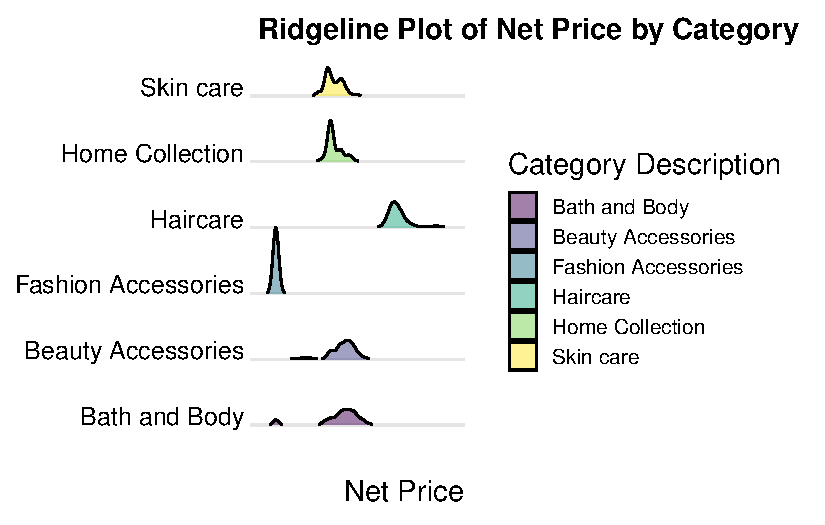
\includegraphics{Time-Serise-EDA_files/figure-pdf/unnamed-chunk-8-1.pdf}

}

\end{figure}

\begin{Shaded}
\begin{Highlighting}[]
\FunctionTok{library}\NormalTok{(tidyverse)}
\FunctionTok{library}\NormalTok{(lubridate)}
\FunctionTok{library}\NormalTok{(data.table)}
\FunctionTok{library}\NormalTok{(ggplot2)}
\FunctionTok{library}\NormalTok{(forecast)}
\FunctionTok{library}\NormalTok{(scales)  }\CommentTok{\# 用于逗号格式化}
\FunctionTok{library}\NormalTok{(tidyverse)}
\FunctionTok{library}\NormalTok{(lubridate)}
\FunctionTok{library}\NormalTok{(data.table)}
\FunctionTok{library}\NormalTok{(ggplot2)}
\FunctionTok{library}\NormalTok{(forecast)}
\FunctionTok{library}\NormalTok{(scales)  }\CommentTok{\# 用于逗号格式化}


\CommentTok{\# 解析日期}
\NormalTok{df}\SpecialCharTok{$}\StringTok{\textasciigrave{}}\AttributeTok{Document Date}\StringTok{\textasciigrave{}} \OtherTok{\textless{}{-}} \FunctionTok{as.Date}\NormalTok{(df}\SpecialCharTok{$}\StringTok{\textasciigrave{}}\AttributeTok{Document Date}\StringTok{\textasciigrave{}}\NormalTok{, }\AttributeTok{format =} \StringTok{"\%m/\%d/\%Y"}\NormalTok{)}

\CommentTok{\# 检查并移除无效日期}
\NormalTok{df }\OtherTok{\textless{}{-}}\NormalTok{ df }\SpecialCharTok{\%\textgreater{}\%}
  \FunctionTok{filter}\NormalTok{(}\SpecialCharTok{!}\FunctionTok{is.na}\NormalTok{(}\StringTok{\textasciigrave{}}\AttributeTok{Document Date}\StringTok{\textasciigrave{}}\NormalTok{))}

\CommentTok{\# 提取年月}
\NormalTok{df }\OtherTok{\textless{}{-}}\NormalTok{ df }\SpecialCharTok{\%\textgreater{}\%}
  \FunctionTok{mutate}\NormalTok{(}\AttributeTok{YearMonth =} \FunctionTok{floor\_date}\NormalTok{(}\StringTok{\textasciigrave{}}\AttributeTok{Document Date}\StringTok{\textasciigrave{}}\NormalTok{, }\StringTok{"month"}\NormalTok{))}

\CommentTok{\# 按年月和销售渠道聚合净价}
\NormalTok{df\_channel\_monthly }\OtherTok{\textless{}{-}}\NormalTok{ df }\SpecialCharTok{\%\textgreater{}\%}
  \FunctionTok{group\_by}\NormalTok{(YearMonth, }\StringTok{\textasciigrave{}}\AttributeTok{Sales Channel}\StringTok{\textasciigrave{}}\NormalTok{) }\SpecialCharTok{\%\textgreater{}\%}
  \FunctionTok{summarise}\NormalTok{(}\AttributeTok{Net\_Price =} \FunctionTok{sum}\NormalTok{(}\StringTok{\textasciigrave{}}\AttributeTok{Net Price}\StringTok{\textasciigrave{}}\NormalTok{, }\AttributeTok{na.rm =} \ConstantTok{TRUE}\NormalTok{)) }\SpecialCharTok{\%\textgreater{}\%}
  \FunctionTok{ungroup}\NormalTok{()}
\end{Highlighting}
\end{Shaded}

\begin{verbatim}
`summarise()` has grouped output by 'YearMonth'. You can override using the
`.groups` argument.
\end{verbatim}

\begin{Shaded}
\begin{Highlighting}[]
\CommentTok{\# 绘制按销售渠道的月度时间序列图,增加Y轴的可读性}
\FunctionTok{ggplot}\NormalTok{(df\_channel\_monthly, }\FunctionTok{aes}\NormalTok{(}\AttributeTok{x =}\NormalTok{ YearMonth, }\AttributeTok{y =}\NormalTok{ Net\_Price, }\AttributeTok{color =} \StringTok{\textasciigrave{}}\AttributeTok{Sales Channel}\StringTok{\textasciigrave{}}\NormalTok{)) }\SpecialCharTok{+}
  \FunctionTok{geom\_line}\NormalTok{() }\SpecialCharTok{+}
  \FunctionTok{labs}\NormalTok{(}\AttributeTok{title =} \StringTok{"Monthly Net Price Over Time by Sales Channel"}\NormalTok{,}
       \AttributeTok{x =} \StringTok{"Date"}\NormalTok{, }\AttributeTok{y =} \StringTok{"Net Price"}\NormalTok{) }\SpecialCharTok{+}
  \FunctionTok{theme\_minimal}\NormalTok{() }\SpecialCharTok{+}
  \FunctionTok{theme}\NormalTok{(}\AttributeTok{legend.position =} \StringTok{"bottom"}\NormalTok{) }\SpecialCharTok{+}
  \FunctionTok{scale\_y\_continuous}\NormalTok{(}\AttributeTok{labels =}\NormalTok{ comma) }\SpecialCharTok{+}  \CommentTok{\# 使用逗号格式化Y轴数值}
  \FunctionTok{scale\_x\_date}\NormalTok{(}\AttributeTok{date\_labels =} \StringTok{"\%Y{-}\%m"}\NormalTok{, }\AttributeTok{date\_breaks =} \StringTok{"2 month"}\NormalTok{)  }\CommentTok{\# 设置X轴显示格式和间隔}
\end{Highlighting}
\end{Shaded}

\begin{figure}[H]

{\centering 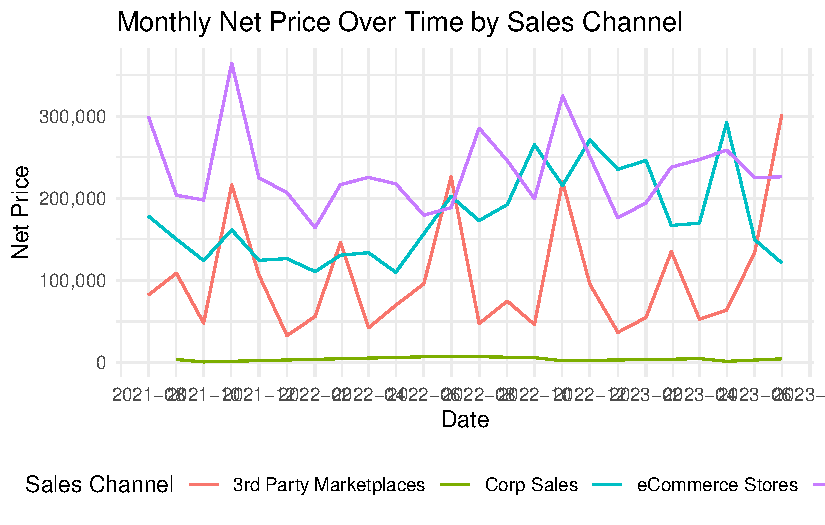
\includegraphics{Time-Serise-EDA_files/figure-pdf/unnamed-chunk-9-1.pdf}

}

\end{figure}



\end{document}
